\documentclass[a4paper]{scrartcl}

\usepackage{amsfonts}
\usepackage{amsmath}
\usepackage{amssymb}
\usepackage{amsthm}
\usepackage{array}
\usepackage[german]{babel}
\usepackage{bm}
\usepackage[pdftex]{color}
\usepackage{enumitem}
\usepackage[utf8]{inputenc}
\usepackage{listings}
\usepackage{tikz}
\usepackage{tikz-cd}
\usepackage{mathrsfs}
\usepackage{mathtools}
\usepackage{url}
\usepackage{verbatim}
\usepackage{xspace}

\usepackage{hyperref}
\usepackage[all]{hypcap}        % Convenience: Let hyperref jump to the figure instead to the caption only.

% Common theorem environments
\theoremstyle{plain}
\newtheorem{theorem}{Theorem}[section]
\newtheorem{theoremdefinition}[theorem]{Theorem/Definition}
\newtheorem{proposition}[theorem]{Proposition}
\newtheorem{propositiondefinition}[theorem]{Proposition/Definition}
\newtheorem{lemma}[theorem]{Lemma}
\newtheorem{Korollar}[theorem]{Korollar}
\newtheorem{fakt}[theorem]{Fakt}

\theoremstyle{definition}
\newtheorem{definition}[theorem]{Definition}
\newtheorem{beispiel}[theorem]{Beispiel}

\theoremstyle{remark}
\newtheorem{bemerkung}[theorem]{Bemerkung}
\newtheorem{notation}[theorem]{Notation}
\newtheorem{motivation}[theorem]{Motivation}

% Include pictures made in inkscape:
\newcommand{\inputhack}{\input}                                         % Rename \input, so that a very simple awk-skript can merge all tex-files.
\graphicspath{{pictures/}}                                              % Set path of the pictures. This is used by the pdf_tex-files generated by inkscape.
\newcommand{\inkpic}[2][\columnwidth]{
  \def\svgwidth{#1}
  \inputhack{pictures/#2.pdf_tex}
}

% Authors and Title
\author{Clelia Albrecht, Felix Boes, Johannes Holke}
\title{Python Skript}
\date{10.\ April 2017 --- 13.\ April 2017}

% Personal Macros
\def\CPP{{\bfseries C\nolinebreak[4]\hspace{-.05em}\raisebox{.4ex}{\tiny\bfseries ++}}\xspace}
\newcommand{\C}{{\bfseries C}\xspace}
\newcommand{\CNeunzig}{{\bfseries C90}\xspace}
\newcommand{\CNeunundneunzig}{{\bfseries C99}\xspace}
\newcommand{\CElf}{{\bfseries C11}\xspace}
\newcommand{\CPPElf}{\CPP{}11\xspace}
\newcommand{\CC}{\C/\CPP}
\newcommand{\Python}{{\bfseries Python}\xspace}
\newcommand{\PythonZwei}{{\bfseries Python2}\xspace}
\newcommand{\PythonDrei}{{\bfseries Python3}\xspace}

% For comments
\newcommand{\todo}[1]{{\color{red}\bfseries Todo: #1 }}
\newcommand{\Felix}[1]{{\color{blue}#1}}

\definecolor{col_cppkeywords}{HTML}{808000}
\definecolor{col_cppclasses} {HTML}{800080}
\definecolor{col_cppmembers} {HTML}{800000}

\lstdefinestyle{CPP}
{
  language=C++,          % Für C++ Listings
  frame=single,
  numbers=left,
  numberstyle=\footnotesize,
  stepnumber=1,
  numbersep=5pt,
  basicstyle=\footnotesize\ttfamily\color{black},
  commentstyle=\itshape\color{gray},
  morekeywords={
    complex,
    int8_t, int32_t, int64_t,
    size_t,
    uint8_t, uint32_t, uint64_t,
  },
  keywords=[2]{
    map,
    ostream,
    std, string,
    unordered_set,
  },
  keywords=[3]{
      basis,
  },
  keywordstyle=\color{col_cppkeywords},
  keywordstyle=[2]\color{col_cppclasses},
  keywordstyle=[3]\color{col_cppmembers},
}
\lstdefinestyle{CPPinline}
{
  language=C++,          % Für C++ Listings
  frame=single,
  numbers=none,
  basicstyle=\ttfamily\color{black},
  commentstyle=\itshape\color{gray},
  morekeywords={
    complex,
    int8_t, int32_t, int64_t,
    size_t,
    uint8_t, uint32_t, uint64_t,
  },
  keywords=[2]{
    map,
    ostream,
    std, string,
    unordered_set,
  },
  keywords=[3]{
      basis,
  },
  keywordstyle=\color{col_cppkeywords},
  keywordstyle=[2]\color{col_cppclasses},
  keywordstyle=[3]\color{col_cppmembers},
}
\newcommand{\lcpp}[1]{\lstinline[style=CPPinline]{#1}}

\definecolor{col_pykeywords}{HTML}{000080}
\definecolor{col_pycomments}{HTML}{808080}
\definecolor{col_pystrings} {HTML}{008000}

\lstdefinestyle{Py}
{
  language=Python,
  frame=single,
  numbers=left,
  numberstyle=\footnotesize,
  stepnumber=1,
  numbersep=5pt,
  basicstyle=\footnotesize\ttfamily\color{black},
  commentstyle=\itshape\color{col_pycomments},
  stringstyle=\bfseries\color{col_pystrings},
  keywordstyle=\bfseries\color{col_pykeywords},
}
\lstdefinestyle{Pyinline}
{
  language=Python,
  frame=single,
  numbers=none,
  basicstyle=\ttfamily\color{black},
  commentstyle=\itshape\color{col_pycomments},
  stringstyle=\bfseries\color{col_pystrings},
  keywordstyle=\bfseries\color{col_pykeywords},
}
\lstdefinelanguage{plain}
{
  frame=single,
  numbers=left,
  numberstyle=\footnotesize,
  stepnumber=1,
  numbersep=5pt,
  basicstyle=\footnotesize\ttfamily\color{black},
}


\newcommand{\lpy}[1]{\lstinline[style=Pyinline]{#1}}

\lstset{
  language=Python,
  style=Py,
  literate={~} {$\bm{\scriptstyle\sim}$}{1}
}

%
% Begin actual document.
%
\begin{document}

\maketitle
\thispagestyle{empty}

\newpage

\thispagestyle{empty}
\null{}\vfill

\begin{center}
  \begin{minipage}{.7\columnwidth}
   Für Mama und Papa
  \end{minipage}
  
  \vspace{3ex}
  
  \hspace{10ex}\begin{minipage}{.7\columnwidth}
   Für Mamma und Papa
  \end{minipage}
  
  \vspace{3ex}
  
  \hspace{4ex}\begin{minipage}{.7\columnwidth}
   Für Mama und Papa
  \end{minipage}
\end{center}
\vfill

\newpage

\thispagestyle{empty}
\null{}\vfill

\begin{center}
  \begin{minipage}{.7\columnwidth}
    Python ist ja ganz nett, aber ist C nicht besser und überhaupt was soll dieses Einrücken?\\[3ex]
    
    \raggedleft
    \emph{Guido von Rossum}
  \end{minipage}
\end{center}
\vfill

\newpage

\tableofcontents

\newpage

\section{Einleitung}
\label{section:intro}

Bei vielen Anwendungen in der wissenschaftlichen Programmierung sind übersichtlicher, handlicher Code und eine schnell mögliche 
Implementierung, für die man auf viele verschiedene, bereits vorhandene, gute Bibliotheken zugreifen kann, wichtiger als 
Schnelligkeit und optimierter Speicherverbrauch. 

Wer sehr viel Wert auf die letzten beiden Eigenschaften legt, ist zum Beispiel mit \CC als Programmiersprache der Wahl gut beraten 
(siehe auch die erste Hälfte dieses sehr guten Kurses \cite{joelixC}). In den meisten Fällen bringt einen \Python jedoch schneller ans 
Ziel.

Eine der Hauptmotivationen von \Python ist es, eine besonders übersichtliche, gut lesbare und einfache Programmiersprache zu sein. 
Die Syntax ist deshalb sehr reduziert und \Python kommt mit wenigen Schlüsselwörtern aus. Die überschaubare Standardbibliothek ist leicht 
zu erweitern -- tatsächlich ist einer der größten Vorteile von \Python die große Fülle an bereits existierenden Modulen und Bibliotheken,
die einem als Nutzer sehr viel Zeit bei der Programmierung ersparen können (mehr dazu kann in \textbf{Abschnitt \ref{section:module}}
nachgelesen werden).

Diese Erweiterbarkeit von \Python sorgt auch dafür, dass Nachteile (wie zum Beispiel die im Vergleich zu maschienennäheren Sprachen 
eher langsame Performance) ausgeglichen werden können. Beispielsweise können performancekritische Routinen in \C implementiert 
und in \Python eingebunden werden um die Vorteile beider Sprachen verbinden zu können (zusammengefasst in \textbf{Tabelle 
\ref{tabelle:effizienz}}). 

\begin{table}[ht]
\centering
 \begin{tabular}{|c|c|c|}
   \hline
                               & Code schnell schreiben & Schnellen Code schreiben\\\hline
   \Python                     &           +            &           -             \\
   \CC                         &           -            &           +             \\
   \Python + \C = $\heartsuit$ &           +            &           +             \\
   \hline
\end{tabular}
\caption{Die awesome Effizienzmatrix}
\label{tabelle:effizienz}
\end{table}

\Python ist keine kompilierte, sondern eine interpretierte Sprache. Der aus \CC bekannte Ablauf Code schreiben -- kompilieren -- 
ausführen entfällt also in der Form. Stattdessen wird der Programmcode dem sogenannten \textbf{Interpreter} übergeben. Hierbei hat man 
zwei Möglichkeiten zur Auswahl: entweder man schreibt den Code direkt in den Interpreter, der die einzelnen Codeblöcke daraufhin sofort 
ausführt, oder man übergibt ihm den Code gebündelt in einer Datei (man hat zudem noch die Möglichkeit, diese Datei direkt ausführbar 
zu machen). Mehr zur Nutzung und Installation von \Python findet sich in \textbf{Anhang \ref{section:installation}}. 

Diese Vorlesung und das begleitende Skript haben zum Ziel, in die Programmiersprache \PythonDrei einzuführen. Dabei richten wir uns 
vor allem an Programmiererinnen, die bereits (fortgeschrittene) Erfahrungen in \CC haben. Es ist jedoch auch möglich, die Vorlesung 
ohne weitreichende Programmierkenntnisse zu besuchen. Der Kurs richtet sich an Bachelorstudenten der Mathematik, die begleitenden 
Übungen sind daher meist mathematisch motiviert.

Aufgrund der knappen Zeit besprechen wir in diesem Skript nur einige Grundlagen von \Python.
Der interessierten Leserin legen wir den \Python-Standard \cite{Python2} und \cite{Python3} aufgrund der hohen Präzision sehr ans Herz.
Das Buchprojekt \cite{LottPython}, welches sich ``nur'' auf \PythonZwei bezieht, ist ebenso (vor allem für weniger erfahrene 
Programmiererinnen) zu empfehlen, da es ausführlich ist, viele gute Beispiele enthält und kaum Programmierkenntnisse voraussetzt.

\vspace{1em}

Dieses Skript ist wie folgt aufgebaut:

In \textbf{Abschnitt \ref{section:datamodel}} erklären wir den wesentlichen konzeptionellen Unterschied zwischen \Python und 
\CC, das \Python-Datenmodel, bevor wir in \textbf{Abschnitt \ref{section:crashkurs}} die grundlegenden 
Bausteine von \Python zusammenfassen. Dieser Crashkurs hat vor allem zum Ziel, Besonderheiten der Syntax aufzuzeigen um bereits 
erfahreneren Programmiererinnen den Einstieg in \Python zu erleichtern. Grundlegende Konzepte wie Bedingungen, Schleifen, Ausgabe 
und Funktionen werden nicht konzeptionell wiederholt.

Die Datentypen, mit denen man in \Python am häufigsten arbeitet, werden in \textbf{Abschnitt \ref{section:std_data_types}} behandelt.
Diese umfassen unter anderem Zahlen, Sequenzen, Mengen, Verzeichnisse und den Umgang mit Dateien. Zu jedem Datentyp listen wir die 
wichtigsten Operationen und Funktionen auf.

Einige Erklärungen zum Namespace befinden sich in \textbf{Abschnitt \ref{section:namespacing}}. Diese sind notwendig um den Umgang 
mit Variablen in den folgenden Abschnitten besser verstehen zu können.

\textbf{Abschnitt \ref{section:funktionen}} widmet sich der Syntax von Funktionen in \Python. Neben Funktionsdefinitionen und -aufrufen 
gibt es noch ein paar Bemerkungen zur Erstellung einer \lpy{main}-Funktion in \Python, sowie den Vorteilen die sich ergeben, wenn 
man Funktionen als Objekte auffasst.

Neben Funktionen sind Klassen eine weitere Möglichkeit, Code übersichtlicher zu gestalten und einfacher nutzbar zu machen. Genauere 
Erklärung zur Syntax, Aufbau und Nutzung von Klassen finden sich in \textbf{Abschnitt \ref{section:klassen}}.  

Ein wichtiger Aspekt des Programmierens ist die Fehlerbehandlung. Diese wird in \Python durch Ausnahmebehandlung vereinfacht, die in 
\textbf{Abschnitt \ref{section:ausnahmen}} ausführlich besprochen wird.

Wie bereits in der Einleitung erwähnt ist einer der größten Vorteile von \Python die riesige Vielfalt an bereits vorhandenen Modulen.
Einen Überblick über der nützlichsten Module die der \Python Standard für Mathematiker bereit hält sowie Anmerkungen zur Nutzung von Modulen 
finden sich in \textbf{Abschnitt \ref{section:module}}.

Zum Abschluss, in \textbf{Abschnitt \ref{section:python_mit_c}} gehen wir noch auf die Möglichkeit ein, bereits vorhandenen 
\CC-Code und sogar bereits kompilierte Bibliotheken mit \Python zu verbinden und somit das beste aus beiden Welten zu vereinen.

In \textbf{Anhang \ref{section:installation}} finden sich zum Schluss noch einige Hinweise zur Installation von 
\Python unter verschiedenen Betriebssystemen.


\newpage

\section{Das Python Datenmodell}
\label{section:datamodel}
Ein wesentlicher Unterschied zwischen \CC und \Python ist das Verhalten von Daten im Speicher und den Zugriff darauf.
Um den Unterschied zu \CC klarer zu machen, beginnen wir mit einer kurzen Wiederholung


\subsection{Wiederholung: Daten in C und C++}
\label{section:datamodel:cc}
In \CC gibt es Variablen.
Diese bestehen aus einer ``Speicheradresse'', einem ``Typ'' und dem dort gespeicherten ``Wert''.
Sie verhalten sich also wie ein zusammenhängendes Stück Speicher, indem ein Wert gespeichert wird und wir wissen, wie wir diesen Wert zu interpretieren haben.
Nehmen wir beispielsweise folgende Codezeile.
\begin{lstlisting}[style=CPP]
int32_t a = 0;
int32_t b = 3;
a = b;
\end{lstlisting}
In der ersten Zeile erstellen wir eine Variable vom Typ \lcpp{int32_t}, d.h.\ wir haben nun ein zusammenhängendes Stück Speicher indem der Wert einer ganzen 32-bit-Zahl gespeichert werden kann,
und legen dort den Wert der Expression \lcpp{0} ab.
In der zweiten Zeile erstellen wir eine weitere Variable vom Typ \lcpp{int32_t} und legen dort den Wert der Expression \lcpp{3} ab.
In der dritten Zeile legen wir den Wert der Expression \lcpp{b} in den zu \lcpp{a} gehörigen Speicher ab.
Nun ist der in \lcpp{a} gespeicherte Wert \lcpp{3} und der in \lcpp{b} gespeicherte Wert ebenfalls \lcpp{3}.
Wenn \lcpp{b} stattdessen vom Typ \lcpp{double *} wäre, führte Zeile 3 zu einem Compilerfehler.


\subsection{Daten in Python}
\label{section:datamodel:python}
Das \Python Datenmodell ist intelektuell nicht so einfach zu fassen wir das Datenmodell von \CC.
Es ist zwar keine Magie, dennoch kann es einige Tage oder gar Wochen dauern kann, bis man sich daran gewöhnt hat.

In \Python gibt es ``Objekte'' und ``Variablen''.
Objekte repräsentieren Daten und Variablen referenzieren auf Objekte.
Zunächst besprechen wir Objekte genauer und kümmer uns im Anschluss um Variablen.


\subsubsection{Objekte}
\label{section:datamodel:python:objekte}
Objekte bestehen aus einer ``Identität'', einem ``Typ'' und einem ``Wert''.
Sie verhalten sich wie ein zusammenhängendes Stück Speicher, in dem ein Wert gespeichert wird,
also ganz genauso wie sich Variablen in \CC verhalten.
Die Identität eines (existierenden) Objekts ändert sich nie und bestimmt ein Objekt (während der Laufzeit) eindeutig.
Wenn man mag, kann man sich die Identität wie die Speicheradresse des Objekts vorstellen (auch wenn man in \Python keine Pointer verwendet).

Ein jedes Objekt ist entweder ``mutable'' und kann nach seiner Erzeugung verändert werden oder es ist ``immutable'' und ist nach seiner Erzeugung konstant.
Dieses Konzept gibt es ebenfalls in \CC:
Alle Typen in \CC sind ohne weiteres ``mutable'', es sei denn, sie bekommen das Präfix \lcpp{const} bei ihrer Definition, denn dann sind sie ``immutable''.

In \Python sind folgende Objekte immutable:
die ganze Zahl \lpy{3} (siehe Abschnitt \ref{section:std_data_types:zahlen}),
das Tupel \lpy{(1, 'a')} (siehe Abschnitt \ref{section:std_data_types:sequenzen}) und
der leere Typ \lpy{None} (siehe Abschnitt \ref{section:std_data_types:none}).
Die folgenden Objekte sind mutable:
Die Liste \lpy{[1, 'a']} (siehe Abschnitt \ref{section:std_data_types:sequenzen}),
das Verzeichnis \lstinline[style=Pyinline]|{ 'Felix' : 405, 'Jonathan' : 599  }| (siehe Abschnitt \ref{section:std_data_types:verzeichnisse})
und die meisten Klassen (siehe Abschnitt \ref{section:klassen}).


\subsubsection{Variablen}
\label{section:datamodel:python:variablen}
In \Python haben Variablen keinen Typ.
Wir wiederholen nochmal: In \Python haben Variablen keinen Typ.
Und ja, in der Tat, wir wiederholen nochmal: In \Python haben Variablen keinen Typ.
Variablen referenzieren auf Objekte; sie sind sozusagen die (temporären) Namen von Objekten.
Wenn man mag, kann man sich Variablen wie \lcpp{(void)}-Pointer vorstellen (auch wenn man in \Python keine Pointer verwendet).

Variablen beziehen sich immer auf ein Objekt.
Beim Erstellen einer Variable muss ihr konsequenterweise direkt ein Objekt zugewiesen werden.
Betrachten wir ein einfaches Beispiel.
\begin{lstlisting}
a = 'Hallo' # Erstelle a; a referenziert das Objekt 'Hallo'.
b = 'Welt'  # Erstelle b; b referenziert das Objekt 'Welt'.
a = b       # a bezieht sich nun auf das Objekt "Welt".
b = 3.141   # b bezieht sich nun auf das Objekt 3.141
\end{lstlisting}
In der ersten Zeile erstellen wir eine Variable \lpy{a}, die sich auf das Objekt \lpy{'Hallo'} bezieht.
Das Objekt \lpy{'Hallo'} hat beispielsweise die Identität \lpy{1000}.
In der zweiten Zeile erstellen wir eine Variable \lpy{b} die sich auf das Objekt \lpy{'Welt'} bezieht.
Das Objekt \lpy{'Welt'} hat beispielsweise die Identität \lpy{2000}.
In der dritten Zeile weisen wir \lpy{a} die Referenz auf das Objekt zu, auf das sich \lpy{b} bezieht.
In der vierten Zeile weisen wir \lpy{b} die Referenz auf das Objekt \lpy{3.141} zu.
Das Objekt \lpy{3.141} hat beispielsweise die Identität \lpy{3000}.
Danach bezieht sich \lpy{a} auf \lpy{'Welt'} und \lpy{b} auf \lpy{3.141}.

\subsection{Speichermanagement}
Die meisten Objekte können genau solange verwendet werden, wie es Variablen gibt, die auf sie referenzieren.
(Einige Ausnahmen sind beispielsweise Zahlen und das Objekt \lpy{None}.)
Objekte, die nicht mehr verwendet werden können, werden automatisch dem ``Garbage Collector'' übergeben.
Dieser entfernt die Objekte nach eigenem Bedarf aus dem Speicher.
Das ist in den meisten Fällen bequemer als in \CC, wo man seinen Speicher selbst verwalten muss.
In der Zeit wo der \CC Programmierer seinen Speicher aufräumt, trinken wir lieber GLUMP%
\footnote{GLUMP Alkoholcola vereint das erweckende Prickeln von koffeinhaltiger Cola mit der betäubenden Wirkung von Alkohol.}.


\newpage

\section{Crashkurs}
\label{section:crashkurs}
Wir beginnen mit einem Überblick der grundlegende Bausteine.
In den nachfolgenden Kapiteln besprechen wir einige der Bausteine nochmal im Detail.


\subsection{Kommentare}
\label{section:crashkurs:kommentare}
Kommentare in \Python beginnen mit \lpy{#} und enden am Ende der Zeile.
Sie verhalten sich also ganz genau wie Kommentare in \CC, die mit \lcpp{//} beginnen%
\footnote{Die Kommentare \lcpp{//} wurden in \CNeunundneunzig (siehe \cite{C99}) eingeführt.}.
Gut platzierte Kommentare dürfen in keinem Programm fehlen.
Ein schlecht kommentiertes Programm ist ein Anzeichen dafür, dass es von einem schlechten Programmierer geschrieben wurde.


\subsection{Print}
\label{section:crashkurs:print}
So gut wie alle Objekte können durch die \Python Funktion \lpy{print} auf der Standardausgabe ausgegeben werden.
Das liegt daran, dass die meisten Objekte Klassen sind und die Funktion \lpy{__str__} implementieren (auch wenn wir das jetzt noch nicht verstehen; siehe Abschnitt \ref{section:klassen:spezielle_funktionen}).
Die Funktion \lpy{print} ist für \PythonZwei und \PythonDrei verschieden.
\begin{lstlisting}
print 'Hallo', 'Welt'   # Python2
print ('Hallo', 'Welt') # Python3
\end{lstlisting}
In diesem Skript nutzen wir die von \PythonDrei bereitgestellte Version von \lpy{print}.
Will man in \PythonZwei die \lpy{print}-Funktion aus \PythonDrei verwenden, kann man folgende Zeile am Anfang seines Skript einfügen.
\begin{lstlisting}
from __future__ import print_function # Nutze Python3-print in Python2
\end{lstlisting}


\subsection{Typ und Identität}
\label{section:crashkurs:typ_und_id}
Um die Identiät eines Objekts \lpy{x} zu bestimmen, nutzen wir die Funktion \lpy{id(x)}.
Sie gibt einen String zurück, den wir mit \lpy{print} ausdrucken können.
Ganz ähnlich bekommen wir den Typ eines Objekts mit \lpy{type(x)}.


\subsection{Zahlen}
\label{section:crashkurs:zahlen}
In \Python gibt es die Zahlentypen \lpy{int}, \lpy{long}, \lpy{float} und \lpy{complex}.
Sie verhalten sich (fast) genauso wie die aus \CC bekannten Typen \lcpp{int}, \lcpp{long}, \lcpp{float} und \lcpp{complex}%
\footnote{Der Typ \lpy{complex} wurde in \CNeunundneunzig (siehe \cite{C99}) eingeführt.}.
Man erstellt ein Objekt vom Typ \lpy{int}, durch Angabe einer ganzen Zahl oder durch Aufrufen der Funktion \lpy{int}.
Ähnlich erstellt man ein Objekt vom Typ \lpy{float}, durch Angabe einer Kommazahl oder durch Aufrufen der Funktion \lpy{float}.
\begin{lstlisting}
print( 2 )        # 2    typ: int
print( int(2.1) ) # 2    typ: int
print( 2.0 )      # 2.0  typ: float
print( float(2) ) # 2.0  typ: float
\end{lstlisting}
Man kann zwei verschiedene oder gleiche Zahlentypen mit mathematischen Operatoren verbinden.
Das Ergebnis hat den ``genaueren'' Typ.
Des Weiteren beschreibt \lpy{//} die ganzzahlige Division ohne Rest.
\begin{lstlisting}
print( 2 + 3.3 )  # 5.3  typ: int +  float -> float
print( 5 // 2 )   # 2    typ: int // int   -> int
print( 5.3 // 2 ) # 2.0  typ: int // float -> float
\end{lstlisting}
Die Division von Ganzzahlen unterscheidet sich in \PythonZwei und \PythonDrei.
\begin{lstlisting}
4 /  2 # Python2: 2 vom Typ int;   Python3: 2.0 vom Typ float;
4 // 2 # Python2: 2 vom Typ int;   Python3: 2   vom Typ int;
\end{lstlisting}


\subsection{Strings}
\label{section:crashkurs:strings}
Strings die eine Zeile lang sind, werden entweder mit \lpy{'} oder mit \lstinline[style=PyInline]|"| begonnen und beendet.
Soll ein String mehre Zeilen lang sein, kann man ihn mit \lstinline[style=PyInline]|"""| beginnen und beenden.
Genau wie in \CC gibt es gewisse Zeichen, die nicht direkt geschrieben werden können und mit \lstinline[language=C++,style=CPP]|\| beginnen müssen (zum Beispiel werden neue Zeilen durch \lstinline[language=C++,style=CPP]|\n| ausgedrückt).
Folgender Code erstellt den String ``Hallo[Neue Zeile]Welt''.
\begin{lstlisting}
print( 'Hallo\nWelt' ) # Hallo[neue Zeile]Welt
\end{lstlisting}
Es gibt eine große Auswahl an Funktionen, um aus einem gegebenen String einen neuen zu erstellen.
Beispielsweise verknüpft man zwei Strings mit \lpy{+} und die Funktion \lpy{lower} ersetzt alle Großbuchstaben durch Kleinbuchstaben.
\begin{lstlisting}
print( 'Hallo' + ' ' + 'Welt' ) # Hallo Welt
print( 'Hallo Welt'.lower() )   # hallo welt
\end{lstlisting}


\subsection{Bedingungen}
\label{section:crashkurs:bedingungen}
In \Python gibt es genau zwei Objekte \lpy{True} und \lpy{False} von Typ \lpy{bool}.
(Fast) alle Typen können mit der Funktion \lpy{bool} in einen der beiden Objekte umgewandelt werden.
Den Kontrollfluss des Programms steuert man im einfachsten Fall wir folgt.
\begin{lstlisting}
if bedingung:
  ausdruck
  ...
\end{lstlisting}
Das heißt, wir brauchen zunächst eine Expression \lpy{bedingung}, die als \lpy{True} oder \lpy{False} interpretiert werden kann.
Wertet sie als \lpy{True} aus, so wird ein Block von Ausdrücken ausgeführt.
Anders als in \CC werden in \Python Blöcke nicht durch Klammern, sondern durch konsistente Einrückung definiert.
\begin{lstlisting}
x = 101//3+46//5
if x == 42:
  print('Die Antwort')
\end{lstlisting}
Da gut eingerückter Code (also Code, in dem jeder Block konsistent eingerückt ist) deutlich lesbarer sind als nicht eingerückter
Code, ist er in jedem Fall -- unabhängig von der Sprache -- ein Zeichen für eine gute Programmiererin. 

Da es jedoch trotzdem immer noch genug Leute gibt, die hässlichen Code produzieren, wird man in \Python dazu gezwungen, auf 
konsistente Einrückung zu achten: zu einem Block gehören genau die nachfolgenden Zeilen, die genauso weit eingerückt sind wie die 
erste Zeile des Blocks. Bei nicht konsistenter Einrückung gibt es Syntaxfehler. Dies macht es sehr schwer, hässlichen Code in
\Python zu schreiben.

Aus eigener Erfahrung können wir sagen, dass man sich als erfahrene \CC Programmiererin recht schnell an diese Konvention gewöhnen kann, 
wenn man auch schon vorher auf sauber geschriebene Programme geachtet hat.

Optional besteht eine Bedingung aus keinem oder mehreren \lpy{elif bedingung:}\footnote{sprich ``else if''} und keinem oder einem \lpy{else:}
Die Konstrukte \lpy{else:} und \lpy{elif bedingung:} in \Python verhalten sich wie die Konstrukte \lcpp{else} und \lcpp{else if} in \CC.
\begin{lstlisting}
x = 101//3+46//5               # x = ?
if x == 42:                    # Falls x den Wert 42 hat:
  print('Die Antwort')         # Drucke 'Die Antwort'
elif x == 84:                  # Sonst, falls x den Wert 84 hat:
  print('Zweimal die Antwort') # Drucke 'Zweimal die Antwort'
elif x == 106:                 # Sonst, falls x den Wert 106 hat:
  print('Dreimal die Antwort') # Drucke 'Dreimal die Antwort'
else:                          # In allen anderen Faellen:
  print('Versuchs nochmal')    # Drucke 'Versuchs nochmal'
\end{lstlisting}


\subsection{Listen}
\label{section:crashkurs:listen}
In \Python gibt es verschiedene ``Containertypen'' und hier besprechen wir den Typ \lpy{list}.
Eine Liste \lpy{thor} ist eine linear geordnete Menge von Variablen, auf die man mit \lpy{thor[0], thor[1], ..., thor[i]} zugreift.
Um auf Elemente von hinten zuzugreifen, sind negative Werte für \lpy{i} erlaubt.
\begin{lstlisting}
thor = [2, 'Hallo', 33.3, 'Welt', [] ] # Erzeugt eine Liste
print( thor[1], thor[-1] )             # Gibt folgendes aus: Hallo []
\end{lstlisting}
Die Länge einer Liste ist \lpy{len(thor)}.
Listen sind mutable, das heißt wir können sie verändern.
Mit \lpy{thor.append(x)} erweitert man die Liste \lpy{thor} um die Variable \lpy{x} und mit \lpy{thor.remove(x)} entfernt man die erste Variable mit dem Wert \lpy{x}.
Ob ein Objekt mit Wert \lpy{x} in \lpy{thor} enthalten ist, testet man mit \lpy{x in thor}.
Mit \lpy{thor+asgard} verknüpft man die beiden Listen \lpy{thor} und \lpy{asgard}.


\subsection{Schleifen}
\label{section:crashkurs:schleifen}
In \Python gibt es zwei Arten von Schleifen.
Die \lpy{while}-Schleife führt einen Codeblock aus, solange die vor der Ausführung des Blocks geprüfte Bedingung als \lpy{True} auswertet.
\begin{lstlisting}
while bedingung:
  ausdruck
  ...
\end{lstlisting}
Da uns dieses Konzept aus \CC sehr vertraut ist, brauchen wir hier kein Beispiel.

Die \lpy{for}-Schleife führt einen Codeblock für jedes Element einer gegebenen Sequenz (siehe Abschnitt \ref{section:std_data_types:sequenzen}) aus.
Eine Sequenz kann zum Beispiel eine Liste oder ein String sein.
\begin{lstlisting}
for i in s: # der Ausdruck s muss als Sequenz interpretiert werden koennen
  ausdruck
  ...
\end{lstlisting}
Dabei referenziert die Laufvariable \lpy{i} jedes Element der Sequenz \lpy{s} nacheinander einmal. Durch Verwendung von \lpy{i} innerhalb 
des folgenden Codeblocks kann 
dann auf den Wert des jeweiligen Objekts zugegriffen werden. Nach Ausführung des Codeblocks der \lpy{for}-Schleife referenziert 
\lpy{i} dann das nächste Element von \lpy{s}, bis das Ende der Sequenz erreicht ist. 

Dies wird durch das folgende Beispiel veranschaulicht:
\begin{lstlisting}
s = 'Hallo Welt' # Die Sequenz 'Hallo Welt'
for i in s:      # Nimm alle i = H,a,l,l,o, ,W,e,l,t
  print(i)       # Drucke i aus
\end{lstlisting}
Hier ist unsere Sequenz \lpy{s} ein String mit dem Wert \lpy{Hallo Welt}. In der \lpy{for}-Schleife nimmt die Laufvariable nacheinander
die Werte der einzelnen Zeichen von \lpy{s}, also \lpy{H,a,l,} \lpy{l,o, ,W,e,l} und \lpy{t}. Im zur Schleife gehörenden Block werden 
diese Zeichen dann einzeln ausgegeben.

Wenn der Codeblock für eine aufsteigende Folge von Zahlen \lpy{from, from+1, ..., to-1} ausgeführt werden soll, nimmt man die Sequenz \lpy{range(from, to)}.
Wichtig ist, dass wir das halboffene Interval betrachten, also nur bis \lpy{to-1} und nicht bis \lpy{to} gehen.
Damit verhält sich der \Python-Code \lpy{for i in range(from, to):} ganz genau wie der \CC-Code \lstinline[language=C++,style=CPPinline]|for(i = from; i < to; ++i) { ... }|.
Hier ein Beispiel
\begin{lstlisting}
sum = 0              # Setze sum auf 0
for i in range(1,5): # Nimm alle i = 1, 2, 3, 4
  sum += 3*i         # Addiere 3*i zu sum
print( sum )         # Drucke sum aus
\end{lstlisting}

Will man eine absteigende Folge ganzer Zahlen, oder allgemeiner eine Folge ganzer Zahlen mit Schrittweite \lpy{step > 0} oder \lpy{step < 0} haben,
nimmt man die Sequenz \lpy{range(from,to,step)}.
Also können wir obiges Beispiel wie folgt umformulieren.
\begin{lstlisting}
sum = 0                  # Setze sum auf 0
for i in range(3,15, 3): # Nimm alle i = 3, 6, 9, 12
  sum += i               # Addiere i zu sum
print( sum )             # Drucke sum aus
\end{lstlisting}


\subsection{Funktionen}
\label{section:crashkurs:funktionen}
Meistens will man sich wiederholende Codeblöcke auslagern und natürlich kann man auch in \Python Funktionen definieren.
Jede Funktionsdefinition erstellt ein Objekt, welches der Funktion im Speicher entspricht.
Außerdem wird eine Variable definiert, welche auf die Funktion im Speicher referenziert.
\begin{lstlisting}
def funktionsname(parameter):
  ausdruck
  ...
\end{lstlisting}
Die Variable ist hier \lpy{funktionsname} und zeigt auf das Objekt, welches der definierten Funktion entspricht.

Anders als in \CC hat eine Funktion keine Signatur und keinen definierbaren Rückgabetyp.
Mit \lpy{return} können kein, ein oder mehrere Objekte zurückgegeben werden.
Wird kein Objekt zurückgegeben, so ist die Rückgabe automatisch \lpy{None}.
Wird ein Objekt \lpy{x} zurückgegeben, so ist der Rückgabetyp automatisch \lpy{type(x)}.
Werden mehrere Objekte zurückgegeben, so werden diese automatisch in einem \lpy{tuple} zusammengefasst, der Rückgabetyp ist also \lpy{tuple}.
Ein Tuple ist eine Liste, die nicht geändert werden kann (siehe Abschnitt \ref{section:std_data_types:sequenzen}).
\begin{lstlisting}
def f(i):
  if i == 1:
    return 1           # Rueckgabetyp: int,   Rueckgabewert: 1
  elif i == 2:
    return 'Hallo', 44 # Rueckgabetyp: tuple, Rueckgabewert: ('Hallo', 44)

print( type( f ) )                 # <class 'function'>
print( type( f(1) ) )              # <class 'int'>
print( type( f(2) ) )              # <class 'tuple'>
print( type( f('Gurkenwasser') ) ) # <class 'NoneType'>
\end{lstlisting}
Also ist das von \lpy{f(3)} oder auch \lpy{f('Gurkenwasser')} zurückgegebene Objekt \lpy{None}.

Beim Funktionsausruf übergibt man die Parameter entweder in der Reihenfolge wie sie in der Funktionsdefinition spezifiziert sind, oder man übergibt \lpy{parametername=ausdruck}.
Außerdem kann man den Argumenten einer Funktion Standardwerte übergeben.
Beim Funktionsausruf muss man die Argumente mit Standardwerten nicht angeben, kann es aber.
\begin{lstlisting}
def plus(a,b=1):
  return a+b

plus(4,5)      # = 9
plus(b=5, a=4) # = 9
plus(3)        # = 4
\end{lstlisting}


\subsection{Module}
\label{section:crashkurs:module}
Was \Python wirklich mächtig macht, ist nicht die Sprache an sich, sondern die schier unendliche Fülle an Paketen die \Python-Programmierer bereit stellen.
Ein Modul ist so etwas wie eine ``shared library'' in \CC.
Man kann sie importieren und dann nutzen, die Implementierung haben andere bereits übernommen (siehe Abbildung \ref{figure:xkcd_python}).
\begin{figure}[ht]
  \centering
  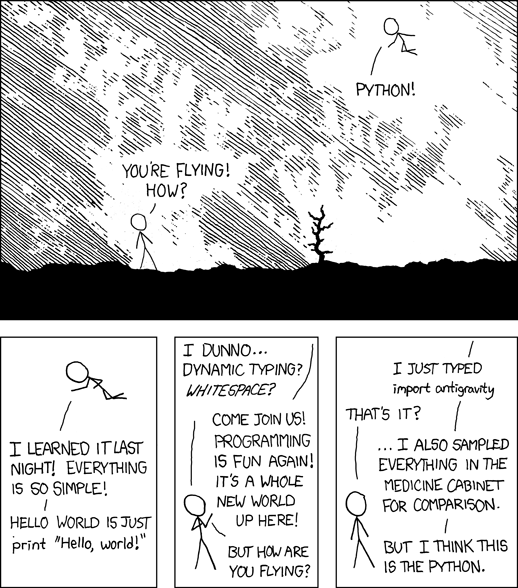
\includegraphics[width=0.5\textwidth]{pictures/xkcd_python.png}
  \caption{\label{figure:xkcd_python}``Python'' by Randall Munroe \cite{Munroe_python}}
\end{figure}

Ein Modul bindet man mit \lpy{import modulname} in sein Programm ein.
Alle Objekttypen (Klassen, Funktionen und andere Objekte) die \lpy{modulname} bereitstellt, können durch \lpy{modulname.oname} erreicht werden.
\begin{lstlisting}
import math
print( math.sin(math.pi/3.0) )
\end{lstlisting}
Wenn man aus \lpy{modulname} bestimmte Objekte einbinden möchte, nutzt man folgende Codezeile.
\begin{lstlisting}
from modulname import oname1, oname2, ...
\end{lstlisting}
Jetzt kann man auf die Objekte direkt (also ohne das Präfix \lpy{modulname.}) zugreifen.
Wir hatten bereits gesehen, wie man die \PythonDrei Printfunktion in \PythonZwei einbinden kann.
\begin{lstlisting}
from __future__ import print_function
\end{lstlisting}
Hier noch ein Beispiel.
\begin{lstlisting}
from math import sin, cos, pi
print( sin(pi/3.0), cos(pi/3.0) )
\end{lstlisting}

An dieser Stelle machen wir noch auf Abschnitt \ref{section:module:empfohlene_module} indem wir eine Hand voll \Python-Pakete erwähnen, die wir oft benutzen.


\subsection{Workflow}
\label{section:crashkurs:workflow}
Wir arbeiten recht erfolgreich mit folgendem Workflow.

Beginne ein Projekt in \Python.
Solange du noch nicht fertig bist:
Wenn eine Funktion zu aufwendig zu implementieren ist, suche nach einer bereits vorhandene \Python Bibliothek (es gibt bestimmt eine).
Wenn eine Funktion für dein Projekt zu langsam ist, schreibe sie in \CC und binde sie als Modul ein.
Wie genau letzteres geht, lernen wir noch.


\newpage

\section{Einige Standarddatentypen}
\label{section:std_data_types}
In diesem Abschnitt besprechen wir einige Standarddatentypen, die \Python bereit stellt.
In den darauf folgenden Abschnitten besprechen wir ``Funktionen'' und ``Klassen'' und ``Module''.

\subsection{Zahlen}
\label{section:std_data_types:zahlen}
In \Python gibt es die numerischen Typen \lpy{int}, \lpy{bool}, \lpy{float} und \lpy{complex}.
Objekte dieses Typs sind immer ``immutable''.

Die \Python-Typen \lpy{int}, \lpy{float} und \lpy{complex} verhalten sich ähnlich wie die \CC-Typen \lcpp{int}, \lcpp{float} und \lcpp{complex}.
Hier die wichtigsten Operationen.
\begin{lstlisting}
x + y  # Summe von x und y
x - y  # Differenz von x und y
x * y  # Produkt von x und y
x / y  # Quotient von x and y
x // y # Abgerundeter Quotient x und y
x % y  # Rest von x / y
-x     # Negiere x
+x     # Tut nichts
x ** y # x hoch y
abs(x) # Betrag von x
int(x) # Erstellt int aus x
float(x)        # Erstellt float aus x
complex(re, im) # Erstellt complex aus re und im
divmod(x, y)    # Das Paar (x // y, x % y)
\end{lstlisting}
Die Division von zwei Ganzzahlen wieder eine Ganzzahl in \PythonZwei und eine Gleitkommazahl in \PythonDrei.
Sind die Typen der Operationen verschieden, verhält sich \Python ebenfalls wie \CC und nimmt immer den genaueren Typ.
\begin{lstlisting}
2   /  3   # = 0 in Python2; 0.6666666666666666 in Python3
2   /  3.0 # = 0.6666666666666666
2.0 /  3   # = 0.6666666666666666
2.0 // 3.0 # = 0.0
\end{lstlisting}

Des Weiteren gibt es für \lpy{int}, \lpy{float} und \lpy{complex} typenspezifische Funktionen.
Für \lpy{int} gibt es beispielsweise Bitoperationen \lstinline[style=PyInline]|~|, \lpy{|}, \lpy{&}, \lstinline[style=PyInline]|^|, \lpy{<<} und \lpy{>>};
für \lpy{float} gibt es beispielsweise die Funktion \lpy{as_integer_ration}, die \lpy{x} als Bruch darstellt;
und komplexe Zahlen können beispielsweise mit der Funktion \lpy{conjugate} ihr Komplexkonjugiertes zurückgeben.
Mehr solcher Funktionen sind hier zu finden \cite[Library, Build-in Types, Numeric Types]{Python3}.

Die Funktion \lpy{float(x)} erstellt aus \lpy{x} ein Objekt vom Typ \lpy{float}.
Praktischerweise ist der Typ des Objekts \lpy{x} fast unbeschränkt.
Hier ein Beispiel.
\begin{lstlisting}
float(700)           # Erzeugt das Objekt 700.0
float('   -12345\n') # Erzeugt das Objekt -12345.0
float('1e-003')      # Erzeugt das Objekt 0.001
float('+1E6')        # Erzeugt das Objekt 1000000.0
float('-Infinity')   # Erzeugt das Objekt -inf
\end{lstlisting}
An dieser Stelle sei noch gesagt, dass ein Objekt vom Typ \lpy{typ} genau dann als \lpy{float} (bzw.\ \lpy{int} oder \lpy{complex}) interpretiert werden,
wenn die zu \lpy{typ} gehörige Klasse über die speziellen Memberfunktion \lpy{__float__} (bzw.\ \lpy{__int__} oder \lpy{__complex__}) verfügt.
Was das genau heißt, wird im Abschnitt \ref{section:klassen} erklärt.

\subsection{bool}
\label{section:std_data_types:bool}
Es gibt genau zwei Objekte vom Typ \lpy{bool}.
Sie sind durch ihren Wert \lpy{True} und \lpy{False} eindeutig bestimmt.
Außerdem sind sie immutable.

Als \lpy{False} interpretiert \Python die folgende Werte:
Zahlen \lpy{0} und \lpy{0.0};
leere Mengen (ja, leere Menge{\bfseries n}, i.e.\ Objekte vom Typ \lpy{set}, deren Wert mit dem Wert \lstinline[style=Pyinline]|{}| übereinstimmt (selbst wenn ihre Identitäten verschieden sind));
leere Sequenzen \lpy{''}, \lpy{()} und \lpy{[]};
und leere Verzeichnisse.
Allgemein kann man ein Objekt vom Typ \lpy{x} genau dann als \lpy{bool} interpretiert werden, wenn die zu \lpy{x} gehörige Klasse über eine Memberfunktion \lpy{__bool__} verfügt.
Was das genau heißt, wird im Abschnitt \ref{section:klassen} erklärt.

Es gibt folgende boolschen Operationen.
\begin{lstlisting}
x or  y # y wird nur ausgewertet wenn x False ist
x and y # y wird nur ausgewertet wenn x True ist
  not x # False wenn x True ist und True wenn x False ist
\end{lstlisting}

\subsection{Sequenzen}
\label{section:std_data_types:sequenzen}
Sequenzen sind sogenannte ``Container'', die sich zum Teil ähnlich wie die aus \CC bekannten Arrays verhalten.
Die wichtigsten Sequenztypen sind der mutable Typ \lpy{list}, sowie die immutable Typen \lpy{tuple} und \lpy{str}.


\subsubsection{Gemeinsamkeiten}
\label{section:std_data_types:sequenzen:gemeinsamkeiten}
Besprechen wir zunächst die wichtigsten Operationen, die sich die drei Typen \lpy{list}, \lpy{tuple} und \lpy{str} teilen.
\begin{lstlisting}
a = [x,y,z] # a ist Typ list  mit a[0]=x, a[1]=y, a[2]=z
a = (x,y,z) # a ist Typ tuple mit a[0]=x, a[1]=y, a[2]=z
a = 'xyz'   # a ist Typ str   mit a[0]=x, a[1]=y, a[2]=z
a[i]        # Die Variable a[i]
len(a)      # Laenge von a
\end{lstlisting}
Für nicht-negative Ganzzahlen \lpy{i} ist völlig klar was damit gemeint ist.
Allerdings sind auch negative Werte für \lpy{i} zulässig: hier benutzt \Python den Index \lpy{len(a) + i}.
Insgesamt sind nur Werte \lpy{-len(a) <= i < len(a)} zulässig.

Um zu überprüfen, ob (der Wert des Objekts der Variable) \lpy{x} mindestens einmal in \lpy{a} vorkommt oder nicht, gibt es die folgenden Operationen.
\begin{lstlisting}
x in a      # True  genau dann wenn x in a enthalten ist
x not in a  # False genau dann wenn x in a enthalten ist
\end{lstlisting}

Um zwei Container desselben Typs (also \lpy{list}, \lpy{tuple} oder \lpy{str}) hintereinander zu heften gibt es folgende Operationen.
Dabei entsteht immer ein neues Objekt.
\begin{lstlisting}
a + b # Erstelle die Verkettung von a und b (erst a dann b)
n * a # a + a + ... + a (n mal)
\end{lstlisting}
Beispielsweise erstellt man eine Liste der Größe \lpy{n} mit Einträgen \lpy{0} wie folgt.
\begin{lstlisting}
thor = n*[0] # Die Sequenz [0, 0, ...., 0] der Laenge n
\end{lstlisting}

Einen Teilsequenz kann man wie folgt bekommen.
\begin{lstlisting}
b=a[i:j]   # b[t] = a[i+t]   mit i <= i+t   < j
b=a[i:j:k] # b[t] = a[i+t*k] mit i <= i+t*k < j
\end{lstlisting}
Für nicht-negative \lpy{i} und \lpy{j} ist völlig klar was damit gemeint ist.
Auch hier sind negative Werte für \lpy{i} und \lpy{j} zulässig solange \lpy{-len(a) <= i,j < len(a)} erfüllt ist.
\begin{lstlisting}
a[2:-4] # Die Variablen a[2], ..., a[n-4] fuer n = len(a)
\end{lstlisting}
Außerdem können \lpy{i} und \lpy{j} weggelassen werden.
Dann ist \lpy{i = 0} bzw.\ \lpy{j = len(a)}.
\begin{lstlisting}
a[ :-4] # Die Variablen a[0], ..., a[n-4] fuer n = len(a)
a[2:  ] # Die Variablen a[2], ..., a[n]   fuer n = len(a)
\end{lstlisting}
Bei diesen Teilsequenzen ist es wichtig zu wissen, dass hier sogenannte ``oberflächeliche Kopien'' erstellt werden.
Was das ist und welche (ungeahnten) Konsequenzen das haben kann, behandeln wir im Abschnitt \ref{section:std_data_types:sequenzen:kopien}.

Weitere nützliche Operationen sind die Folgenden.
\begin{lstlisting}
min(a)     # Kleinstes Element von a, falls sinnvolle Frage
max(a)     # Groesstes Element von a, falls sinnvolle Frage
a.count(x) # Anzahl der Variablen die gleich x sind.
a.index(x) # Index von der ersten Variablen, die gleich x ist
a.index(x, i)    # Index von der ersten Variablen, die gleich x ist sowie
                 # gleich oder nach i kommt
a.index(x, i, j) # Index von der ersten Variablen, die gleich x ist sowie
                 # gleich oder nach i sowie vor j kommt
\end{lstlisting}


\subsubsection{Oberflächeliche und tiefe Kopien}
\label{section:std_data_types:sequenzen:kopien}
Eine Sequenz ist ein Objekt.
Der Wert einer Sequenz ist eine linear geordnete Menge von Variablen.
Ja richtig, der Wert einer Sequenz ist eine linear geordnete Menge von Variablen (und nicht von Objekten).
Deshalb ist eine sogenannte ``oberflächliche Kopie'' einer Sequenz \lpy{a} ein neues Objekt \lpy{b} mit dem selben Wert wie \lpy{a}.
Das heißt, \lpy{a[0]} und \lpy{b[0]} zeigen auf dasselbe Objekt.
Schauen wir uns das folgende Beispiel an:
\begin{lstlisting}
# In diesem Beispiel bezeichnen wir Listen der Form [i,j] wobei i und j
# Ganzzahlen sind als Vektoren.

# Zuerst erstellen wir eine Liste von drei Vektoren und kopieren die Liste
vekt_lst = [ [0,1], [2,3], [5,1] ] # Liste von drei Vektoren
kopie    = vekt_lst[0:3]           # Oberflaechliche Kopie

# Die Listen sind verschieden
print(id(vekt_lst)) # 140541651867528
print(id(kopie))    # 140541679766536

# Die Elemente von einer der Listen zu aendern hat folgenden Effekt
v = kopie[0] # zeigt auf denselben Vektor wie kopie[0] und vekt_lst[0]
v[0] = 100   # v wird geaendert
print(v)        # [100,1]
print(kopie)    # [[100, 1], [2, 3], [5, 1]]
print(vekt_lst) # [[100, 1], [2, 3], [5, 1]]
\end{lstlisting}

Dieses Verhalten ist in den meisten Fällen gewollt.
Wenn man eine ``tiefe Kopie'' der Sequenz \lpy{a} braucht, also eine Sequenz \lpy{b},
deren ``mutable'' Objekte denselben Wert, aber eine verschiedene Identität haben, dann benutzt man das Modul \lpy{copy}
(siehe auch Abschnitt \ref{section:module:empfohlene_module:copy}).
Das geschieht wie folgt.
\begin{lstlisting}
# In diesem Beispiel bezeichnen wir Listen der Form [i,j] wobei i und j
# Ganzzahlen sind als Vektoren.

import copy

# Zuerst erstellen wir eine Liste von drei Vektoren und kopieren die Liste
vekt_lst = [ [0,1], [2,3], [5,1] ] # Liste von drei Vektoren
kopie    = copy.deepcopy(vekt_lst) # Tiefe Kopie

# Die Listen sind verschieden
print(id(vekt_lst)) # 140541651867528
print(id(kopie))    # 140541679766536

# Die Elemente von einer der Listen zu aendern hat folgenden Effekt
v = kopie[0] # zeigt auf denselben Vektor wie kopie[0]
v[0] = 100   # v wird geaendert
print(v)        # [100,1]
print(kopie)    # [[100, 1], [2, 3], [5, 1]]
print(vekt_lst) # [[  0, 1], [2, 3], [5, 1]]
\end{lstlisting}


\subsubsection{tuple}
\label{section:std_data_types:sequenzen:tuple}
Der Containertyp \lpy{tuple} ist immutable. Das bedeutet, dass weder einzelne Einträge des Tupels verändert werden können, 
noch kann die Länge des Tupels verändert werden. Das Tupel \lpy{(3, 'Harry Potter')} beispielsweise wird über den gesamten Verlauf des 
Programs das Tupel \lpy{(3, 'Harry Potter')} bleiben und kann nicht zu z.B.\ \lpy{(1, 'LotR')} geändert werden. 

Dennoch nutzt man Tupel implizit rechts häufig. Unter anderem können, wie im Crashkurs Abschnitt \ref{section:crashkurs:funktionen} bereits angedeutet, Funktionen 
mehrere Objekte zurückgeben. Diese werden dann zusammen in ein Tupel gepackt, in der Reihenfolge, in der sie nach dem 
\lpy{return}-Statement aufgezählt sind. Das folgende Beispiel veranschaulicht dies:

\begin{lstlisting}
def doppeltupelfkt(x,y)
  return 2*x, 2*y

z = doppeltupelfkt(1,2)
print( z )              # gibt (2,4) aus
\end{lstlisting}

\lpy{z} ist nach Aufrufen der Funktion das Tupel \lpy{(2,4)}, d.h.\ wenn eine Funktion mehrere Objekte zurückgibt, werden sie in 
einem Objekt abgefangen.

Außerdem gibt es für Tupel noch die Möglichkeit der mehrfachen Zuordnung:

\begin{lstlisting}
x_1, x_2, ... , x_n = z # z ist Tupel mit len(z) = n
\end{lstlisting}

Hierbei wird \lpy{z[i-1]} der Variable \lpy{x_i} zugeordnet. Auf diese Weise können auch die Objekte, die eine Funktion 
zurückgibt, in mehreren Variablen abgespeichert werden statt in nur einem Tupel. Dabei muss darauf geachtet werden, dass 
auf der linken Seite der Zuordnung genau so viele Variablen stehen wie das Tupel Elemente hat.

Ansonsten verfügt \lpy{tuple} über keine weiteren (für diesen Kurs bedeutsamen) Operationen --- abgesehen von den Gemeinsamkeiten mit 
anderen Sequenzen, die im vorangegangenen Abschnitt \ref{section:std_data_types:sequenzen:gemeinsamkeiten} beschrieben wurden.


\subsubsection{list}
\label{section:std_data_types:sequenzen:listen}
Den mutable Containertyp \lpy{list} verwendet man in \Python recht oft.
Neben den Operationen, die alle Sequenzen gemeinsam haben, können wir eine gegebene Liste \lpy{a} mit den nachfolgenden Operationen verändern.

Folgende Operationen fügen Objekte hinzu oder entfernen sie.
\begin{lstlisting}
a[i] = x       # Ersetze a[i] durch x
a.insert(i, x) # Fuege x hinter a[i] ein
a.append(x)    # Fuege x am Ende von a ein
x = a.pop([i]) # Erhalte x = a[i] und entferne a[i] aus der list
a.remove(x)    # Entferne die erste Variable mit Wert x
\end{lstlisting}

Folgende Operationen verlängern eine gegebene \lpy{list} mit Namen \lpy{a} um eine (andere) gegebene \lpy{list}.
\begin{lstlisting}
a += t # Verlaengert a mit t
a *= n # Verlaengert a n mal mit sich selbst
\end{lstlisting}
Wir machen darauf aufmerksam, dass \lpy{a+=t} nicht dasselbe ist wie \lpy{a=a+t}.
Der erste Ausdruck verlängert \lpy{a} um \lpy{t}, der zweite Ausdruck erstellt ein neues Objekt mit Wert \lpy{a+t} und danach referenziert \lpy{a} auf dieses Objekt.
Schauen wir uns dazu folgendes Beispiel an.
\begin{lstlisting}
thor = ['Valhalla', 42] # Erstellt thor
print(id(thor))         # 140541679765448
thor += ['Valgrind']    # fuegt 'Valgrind' hinzu
print(id(thor))         # 140541679765448
thor = thor + ['Suppe'] # erstellt neue Liste und nennt sie thor
print(id(thor))         # 140541679767112
\end{lstlisting}

Listen können auch scheibchenweise mit nur einer Operation verändert werden.
\begin{lstlisting}
a[i:j] = t   # Entferne den slice a[i:j] und fuege dort die Liste t ein
del a[i:j]   # Entferne den slice a[i:j]. Aequivalent zu a[i:j] = []
a[i:j:k] = t # Ersetze den slice a[i:j:k] durch die Elemente der Liste t
del a[i:j:k] # Entferne den slice a[i:j:k]
\end{lstlisting}

Außerdem können wir eine Liste leeren oder eine oberflächliche Kopie anfertigen.
Das funktioniert so:
\begin{lstlisting}
a.clear() # Entfernt alle Elemente von a
a.copy()  # Erstellt eine oberflaechliche Kopie von a
\end{lstlisting}
Eine oberflächliche Kopie erstellt eine neue Liste mit denselben Variablen.
Insbesondere sind die referenzierten Objekte der beiden Listen identisch.
Das will man oft, da so eine oberflaechliche Kopie sehr schnell erstellt ist.
Manchmal möchte man aber, dass die Objekte verschieden sind.
Wie das funktioniert, wird im Abschnitt \ref{section:std_data_types:sequenzen:kopien} besprochen.

Für Schleifendurchläufe (oder auch andere Situationen) kann es sinnvoll sein, eine Liste umzudrehen.
Außerdem möchte man Listen sortieren können, sofern das Sinn macht.
Dafür stehen diese beiden vielsagenden Funktionen bereit.
\begin{lstlisting}
a.reverse() # Kehrt a um
a.sort()    # Sortiert a, falls das Sinn macht
\end{lstlisting}
Genauer gesagt kann man eine Liste sortieren, sofern je zwei Elemente \lpy{x} und \lpy{y} der Liste mit \lpy{x < y} verglichen werden können.
Siehe hierzu auch \ref{section:klassen:spezielle_funktionen}.


\subsubsection{range}
\label{section:std_data_types:sequenzen:range}
Ein sogenanntes ``Rangeobjekt'' ist eine immutable Sequenz von aufsteigenden ganzen Zahlen, die sich so ähnlich wie ein Tupel verhält.
Es gibt drei einfache Möglichkeiten ein Rangeobjekt zu erstellen.
Um ein Rangeobjekt der Zahlen \lpy{0 <= i < n} zu erstellen, ruft man die Funktion \lpy{range(n)} auf.
Um ein Rangeobjekt der Zahlen \lpy{m <= i < n} zu erstellen, ruft man die Funktion \lpy{range(m,n)} auf.
Um ein Rangeobjekt der Zahlen \lpy{m <= i*k < n} zu erstellen, ruft man die Funktion \lpy{range(m,n,k)} auf.
\begin{lstlisting}
range(n)     # (0, 1, ..., n-1)
range(m,n)   # (m, m+1, ..., n-1
range(m,n,k) # (m, m+k, ...., m+l*k) mit m+l*k < k <= m+(l+1)*k
\end{lstlisting}
Für \lpy{n}, \lpy{m} und \lpy{k} sind auch negative Werte möglich, solange dabei eine endliche Sequenz von Zahlen erstellt werden kann.


\subsubsection{list comprehension}
\label{section:std_data_types:sequenzen:list_comprehension}
Die sogenannten \emph{list comprehension} ist eine sehr praktische Möglichkeit um aus bereits vorhandenen Sequenzen neue Listen zu erstellen.
Hier ist \lpy{a} eine Sequenz und wir wollen all diejenigen \lpy{x} aus \lpy{a} haben, die eine gewisse Bedingung \lpy{cond(x)} erfüllen.
\begin{lstlisting}
[ x for x in a if cond(x) ]
\end{lstlisting}
Außerdem können wir statt \lpy{x} eine (von \lpy{x}) abhängende) Expression \lpy{expr(x)} in unsere neue Liste stecken.
\begin{lstlisting}
[ expr(x) for x in a if cond(x) ]
\end{lstlisting}
Noch allgemeiner, können wir eine Expression \lpy{expra(x)} verwenden, wenn die Bedingung \lpy{cond(x)} erfüllt ist und im anderen Fall eine Expression \lpy{exprb(x)} verwenden.
\begin{lstlisting}
[ expra(x) if cond(x) else exprb(x) for x in a  ]
\end{lstlisting}

Hier drei Beispiele.
Wir wollen eine Liste aller natürlichen Zahlen $0 \le x < 9$, die nicht durch $4$ teilbar sind.
\begin{lstlisting}
[ x for x in range(10) if x % 4 != 0 ]
\end{lstlisting}
Wir bekommen ein Tupel \lpy{a} und wollen daraus eine Liste all seiner Strings erstellen.
\begin{lstlisting}
a = ('ss', 20 , 'rtt3', 50, 40.2, [344], ('akk', 'er') )
[ x for x in a if type(x) is str ]
\end{lstlisting}
Wir bekommen ein Tupel \lpy{a} der nur Strings enthält.
Wir wollen eine Liste, die alle Strings aus \lpy{a} enthält, außer der String ist \lpy{'Anakonda'}, den wollen wir durch \lpy{'Python'} ersetzen.
\begin{lstlisting}
a = ( 'blau', 'anakonda', 'Strasse', 'Anakonda', '42', 'Anakonda' )
[ x if x is not 'Anakonda' else 'Python' for x in a ]
\end{lstlisting}


\subsubsection{str}
\label{section:std_data_types:sequenzen:str}
Die immutable Sequenz \lpy{str} verfügt über sehr viele selbsterklärende Funktionen.
Zum Beispiel erstellt man aus einem String \lpy{s} mit \lpy{s.lower()} einen String, der nur aus Kleinbuchstaben besteht. 
Wir besprechen nun noch kurz die Funktion \lpy{format} und verweisen den interessierten Leser auf \cite[Library, Build-in Types, Text Sequence Type]{Python3}.

Oft macht es Sinn, einen String durch Einsetzung von Variablen zu erzeugen.
Dabei sollen die Variablen von der Beschreibung des zu entstehenden Strings getrennt sein.
Dieses Konzept sollte von der \C-Funktion \lcpp{printf} bekannt sein.
In \Python kann man das am einfachsten mit der Funktionen \lpy{s.format(...)} erreichen.
Dabei beschreibt \lpy{s} das Aussehen des Strings, also normalen Text sowie Platzhalter \lstinline[style=PyInline]|'{}'| und
die Parameter von \lpy{format} sind die Variablen, die in die Platzhalter eingesetzt werden.
Hier ein Beispiel:
\begin{lstlisting}
text = 'Hallo {}. Ich bin {} Jahre alt.'.format('Welt', 42)
print(text) # Hallo Welt. Ich bin 42 Jahre alt.
\end{lstlisting}


\subsection{None}
\label{section:std_data_types:none}
Es gibt genau ein Objekt \lpy{None} vom sogenannte Typ \lpy{NoneType}.
Man benutzt dieses Objekt um die Abwesenheit eines Werts oder eines Parameters auszudrücken.
Zum Beispiel ist \lpy{None} der Rückgabetyp einer Funktion, die zurückkehrt ohne ein Objekt mit \lpy{return} zurückzugeben.
Hier ein Beispiel:
\begin{lstlisting}
def ich_geb_nix_zurueck():
  print("Ich hab nix")

x = ich_geb_nix_zurueck()
print( type(x) )
\end{lstlisting}

Ganz oft wird \lpy{None} als Standardparameter für optionale Parameter einer Funktion festgelegt.
Damit lässt sich mit ganz leicht prüfen, ob der Benutzer einen optionalen Parameter übergeben hat oder nicht.
Hier ein simples Beispiel:
\begin{lstlisting}
def sprich_falls_du_was_zu_sagen_hast( was=None ):
  if was is None: # Behandle als ob nichts uebergeben wurde
    print("Ich hab nix zu sagen!")
  else:           # Behandle als ob etwas uebergeben wurde
    print("Ich hab was zu sagen: '{}'.".format(was))

sprich_falls_du_was_zu_sagen_hast()     # Ich hab nix zu sagen!
sprich_falls_du_was_zu_sagen_hast(None) # Ich hab nix zu sagen!
sprich_falls_du_was_zu_sagen_hast(42)   # Ich hab was zu sagen: '42'.
\end{lstlisting}


\subsection{Dateien}
\label{section:std_data_types:file}
In \Python ließt und schreibt man in Dateien ganz ähnlich wie in \CC.
Man öffnet eine Datei, ließt oder schreibt und schließt die Datei sobald man sie nicht mehr braucht.

Das Öffnen funktioniert durch Aufrufen der Funktion:
\begin{lstlisting}
open(file, mode='r')
\end{lstlisting}
Dabei ist \lpy{file} der Pfad der zu öffenden Datei und \lpy{mode} ist der sogenannte Modus.
Die wichtigsten Modi fassen wir hier zusammen.
\begin{lstlisting}
'r' # Lesenzugriff
'w' # Schreibzugriff: alter Inhalt wird ueberschrieben
'a' # Schreibzugriff: beginne am Ende der alten Datei
\end{lstlisting}
Will man Lese- und Schreibzugriff haben, hängt man an \lpy{'r'}, \lpy{'w'} oder \lpy{'a'} das Zeichen \lpy{'+'} an.
Also benutzen wir \lpy{'r+'} und \lpy{'w+'} für Lese- und Schreibzugriff, wobei wir am Anfang der Datei anfangen und
wir benutzen \lpy{'a+'} für Lese- und Schreibzugriff, wobei wir am Ende der Datei anfangen.

Eine Datei \lpy{datei} schließt man wie folgt:
\begin{lstlisting}
datei.close() # Schliesse die Datei.
\end{lstlisting}

Es gibt einfache Möglichkeiten um aus einer geöffneten Datei \lpy{datei} zu lesen.
Entweder man ließt sie zeilenweise aus \lpy{datei.readline(size=1)} oder man ließt sie zeichenweise aus \lpy{datei.read(size=1)}.
Insbesondere ließt \lpy{datei.readline()} eine Zeile und \lpy{datei.read()} ließt ein Zeichen.
Praktischerweise verhält sich eine geöffnete Datei wie eine Sequenz, das heißt, wir können sie ganz einfach mit in einer Schleife auslesen.
In folgendem lesen und drucken wir eine Datei zeilenweise aus.
\begin{lstlisting}
datei = open('dateiname.txt', 'r') # Oeffne die Datei 'dateiname.txt'
for zeile in datei:                # Fuer jede Zeile in der Datei
  print(zeile)                     # Drucke die Zeile aus
datei.close()                      # Schliesse die Datei.
\end{lstlisting}

In eine Datei schreiben wir wie folgt:
\begin{lstlisting}
datei.write(string)
datei.writelines(liste_von_strings)
\end{lstlisting}

\subsection{Mengen}
\label{section:std_data_types:mengen}
In Gegensatz zu Sequenzen, die wir im Abschnitt \ref{section:std_data_types:sequenzen} behandelt haben, sind Mengen ``ungeordnete Container''.
Ähnlich wie bei Cantor, verstehen wir unter einer Menge die Zusammenfassung von bestimmten, wohlunterschiedenen Objekten zu einem Ganzen.
Allerdings verhalten sich Mengen in \Python anders als ``mathematische Mengen'' (sie erfüllen zum Beispiel nicht das Extensionalitätsaxiom, i.e.\ sie sind nicht eindeutig durch ihre Elemente bestimmt).
Das spielt in der Praxis keine Rolle und ist gerüchten zu Folge nur für zwangsgestörte Möchtegernmathematiker ein Problem.


\subsubsection{Mengen erzeugen}
\label{section:std_data_types:mengen:mengen_erzeugen}
Eine Menge kann aus einer (möglicherweise) leeren Sequenz erzeugt werden, sofern jedes Element der Sequenz ``hashbar'' ist.
In Abschnitt \ref{section:klassen:hashbare_objekte} erklären wir genauer, was ``hashbare Objekte'' sind.
Für den Moment begnügen wir uns damit, dass die Standardtypen genau dann hashbar sind, wenn sie immutable sind.
Mengen selbst können entweder mutable oder immutable sein.
Die mutable Variante ist \lpy{set}, die immutable Variante ist \lpy{frozenset}.

Um eine Menge zu erzeugen, welche die Objekte \lpy{4}, \lpy{'Python'} und \lpy{None} zu enthält, rufen wir \lpy{set} mit einer Liste oder einem Tuple das diese Elemente enthält auf.
\begin{lstlisting}
s = set( [4, 'Python', None] )
\end{lstlisting}


\subsubsection{Operationen für set und frozenset}
\label{section:std_data_types:mengen:operationen_fuer_set_und_frozenset}
Folgende Operationen verändern die Menge nicht und stehen somit sowohl \lpy{set} als auch \lpy{frozenset} zur Verfügung.
\begin{lstlisting}
len(s)          # Gibt die Anzahl der Elemente zurueck
x in s          # True  gdw x in s vorkommt
x not in s      # False gdw x in s vorkommt
s == t          # True gdw ihre Elemente uebereinstimmen
s.isdisjoint(t) # True gdw s und t disjunkt sind
s <= t          # True gdw s eine Teilmenge von t ist
s < t           # True gdw s eine echte Teilmenge von t ist
s >= t          # True gdw t eine Teilmenge von s ist
s > t           # True gdw t eine echte Teilmenge von s ist
s | t | ...     # Die Vereinigung von s und t und ...
s & t & ...     # Der Schnitt von s und t und ...
s - t - ...     # Die Differenz von s und t und ...
s ^ t           # Die Symmetrische Differenz von s und t
s.copy()        # Erstelle eine oberflaechliche Kopie von s
\end{lstlisting}
Die Konzepte der oberflächlichen und tiefen Kopien sowie die daraus resultierenden Konsequenzen erklären wir in Abschnitt \ref{section:std_data_types:sequenzen:kopien} am Beispiel der Listen.
Analoge Aussagen gelten für Mengen.

An dieser Stelle gehen wir noch ein wenig auf die Gleichheit von Mengen ein.
Wie gesagt, wertet \lpy{s == t} genau dann als \lpy{True} aus, wenn die Elemente von \lpy{s} und \lpy{t} übereinstimmen.
Das heißt aber nicht, dass \lpy{s} und \lpy{t} dieselbe Identität haben, also an der selben Stelle im Speicher stehen.
Hier ein Beispiel.
\begin{lstlisting}
s = set( range(1,11,1) ) # Die Menge {1,2,...,10}
t = set( range(1,11,1) ) # Die Menge {1,2,...,10}
print( s == t )          # True
print( id(s) )           # 139836709444296
print( id(t) )           # 139836709038568
\end{lstlisting}


\subsubsection{Operationen für set}
\label{section:std_data_types:mengen:operationen_fuer_set}
Jede Menge \lpy{s} vom Typ \lpy{set} ist mutable.
Das heißt, \lpy{s} ist ein Objekt, der Wert von \lpy{s} ist die Menge seiner Elemente und wir können den Wert von \lpy{s} verändern.
Dazu stehen uns folgende Operationen bereit.
\begin{lstlisting}
s |= t | ... # Erweitert die Menge s um t, ...
s &= t & ... # Entfernt alle Elmente aus s, die nicht in t,... sind
s -= t | ... # Entfernt alle Elemente aus s, die in t, ... sind
s ^= t       # Entfernt alle Elemente aus s, die nicht gleichzeitig
             # in s und t sind
add(e)       # Erweitert s um e
remove(e)    # Entfernt e aus s; loest KeyError aus, wenn e nicht in s ist
discard(e)   # Entfernt e aus s falls e in s ist
pop()        # Entfernt ein Element aus s und gibt es zurueck
clear()      # Entfernt alle Elemente aus s
\end{lstlisting}

Wir bemerken hier nochmal, dass die Operationen nur den Wert der Menge \lpy{s} verändern, die Identität \lpy{id(s)} bleibt bestehen.
\begin{lstlisting}
s = set( range(1, 6,1) ) # Die Menge {1,2,...,5}
t = set( range(6,11,1) ) # Die Menge {5,6,...,10}
print( id(s) )           # 139836709038792
print( id(t) )           # 139836709444296
s.add(11)                # Fuege zu s das Element 11 hinzu
print( id(s) )           # 139836709038792
print( id(s |  t) )      # 139836709037448
s |= t                   # Fuege zu s die Elemente 5,6,...,10 hinzu
print( id(s) )           # 139836709038792
\end{lstlisting}
Insbesondere sind die Objekte \lpy{s |= t} und \lpy{s = s | t} verschieden.

\subsection{Verzeichnisse}
\label{section:std_data_types:verzeichnisse}
Objekte von Typ \lpy{dict} nennt man ``Verzeichnisse''.
Ein Verzeichnis verhält sich wie eine partiell definierte mathematische Funktion,
deren Definitionsbereich die Menge der ``hashbaren Objekte'' ist und deren Wertebereich die Menge aller Objekte ist.
In anderen Worten:
Genau wie partiell definierte Funktionen, kann man sich ein Verzeichnis \lpy{d} wie eine Menge von Tupeln \lpy{(key, d[key])} vorstellen,
wobei die linke Seite eines jeden Tupels höchstens einmal als linke Seite vorkommt.
Wenn man bei dieser Vorstellung bleibt, sagt man dass \lpy{d} auf \lpy{key} definiert ist, wenn \lpy{d} das Tupel \lpy{(key, d[key])} enthält.
Diejenigen Objekte, auf denen ein Verzeichnis definiert ist, nennt man ``Schlüssel''.
Schlüssel sind immer hashbare Objekte (siehe unten).
Ist \lpy{key} ein Schlüssel einer Liste \lpy{d}, so ist \lpy{d[key]} ein ``Wert'' des Verzeichnisses \lpy{d}.

Noch haben wir nicht erklärt, was hashbare Objekte sind.
Hier sei gesagt, dass alle vom \Python Standard definierten Objekte hashbar sind, sofern sie immutable sind
(also Objekte vom Typ \lpy{int}, \lpy{float}, \lpy{complex}, \lpy{tuple}, \lpy{str}, \lpy{bool} und \lpy{none},
aber nicht \lpy{list} und \lpy{dict}).
Wir erklären hashbare Objekte in Abschnitt \ref{section:klassen:hashbare_objekte}.


\subsubsection{Verzeichnisse erstellen}
\label{section:std_data_types:verzeichnisse:verzeichnisse_erstellen}
Verzeichnisse können auf folgende Arten erstellt werden:
\begin{lstlisting}
# Leere Verzeichnisse
verz1 = {}
print(verz1)
verz2 = dict()
print(verz2)

# Nichtleeres Verzeichnis
verz3 = { key1 : value1, key2 : value2, key3 : value3, ... }
print(verz3)
\end{lstlisting}
\lpy{verz1} und \lpy{verz2} sind leere Verzeichnisse, \lpy{verz3} verdeutlicht die Syntax eines nichtleeren Verzeichnisses. Die 
``Schlüssel''-``Wert''-Paare werden durch Doppelpunkte getrennt, die Paare voneinander durch Kommata. Ein Beispiel für ein nichtleeres 
Verzeichnis könnte folgendermaßen aussehen:
\begin{lstlisting}
#Verzeichnis speichert Telefonnummern:
telefonbuch = {'Mama':1234, 'Papa':1234, 'Tina':4242, 'Peter':'Keine Nummer'}
\end{lstlisting}

Außerdem kann man ein Verzeichnis aus einer Liste von Tupeln erstellen (solange die linke Seite eines jeden Tupels ein hashbares Objekt ist).
Hier ein Beispiel:
\begin{lstlisting}
verz_eins = { 42 : 'Wahrheit', True : 'Wahrheit' }
verz_zwei = dict([(42, 'Wahrheit'), (True, 'Wahrheit')])
print(verz_eins, verz_zwei)
\end{lstlisting}


\subsubsection{Verzeichnisse nutzen}
\label{section:std_data_types:verzeichnisse:verzeichnisse_nutzen}
Mit den folgenden Funktionen, kann man sich die Größe eines Verzeichnisses \lpy{d} ausgeben lassen,
auf Werte zugreifen, sowie (neue) Schlüssel-Wert Paare setzen oder löschen.
\begin{lstlisting}
len(d)        # Groesse des Verzeichnisses
d[key]        # Gibt den Wert d[key] zurueck oder loest eine Ausnahme aus
d.get(key, x) # Gibt den Wert d[key] zurueck falls er existiert. Sonst
              # wird das Paar (key, x) erstellt und x zurueckgegeben.
d[key] = wert # Setzt d[key] auf wert (auch wenn key noch nicht existiert)
del d[key]    # Entfernt (key, d[key]) oder loest eine Ausnahme aus
d.pop(key, x) # Entfernt (key, d[key]) und gibt d[key] zurueck falls es
              # existiert. Sonst wird x zurueckgegeben.
d.popitem()   # Entfernt bel. Paar (key, d[key]) und gibt d[key] zurueck
d.clear()     # Entfernt alle Paare aus dem Verzeichniss.
\end{lstlisting}
Um nachzuschauen, ob ein Schlüssel in einem Verzeichniss \lpy{d} definiert ist oder nicht nutzen wir die folgenden Operationen.
\begin{lstlisting}
key in d      # Gibt True  zurueck gdw key ein Schluessel von d ist
key not in d  # Gibt False zurueck gdw key ein Schluessel von d ist
\end{lstlisting}
Eine oberflächeliche Kopie eines Verzeichnisses \lpy{d} zu erstellen, benutzt man die folgende Operation.
\begin{lstlisting}
d.copy()
\end{lstlisting}
Die Konzepte der oberflächlichen und tiefen Kopien sowie die daraus resultierenden Konsequenzen erklären wir in Abschnitt \ref{section:std_data_types:sequenzen:kopien} am Beispiel der Listen.
Analoge Aussagen gelten für Verzeichnisse.

An dieser Stelle gehen wir noch ein wenig auf die Gleichheit von Verzeichnissen ein.
Der Vergleich \lpy{s == t} wertet genau dann als \lpy{True} aus, wenn die Paare von \lpy{s} und \lpy{t} übereinstimmen.
Das heißt aber nicht, dass \lpy{s} und \lpy{t} dieselbe Identität haben, also an der selben Stelle im Speicher stehen.
Hier ein Beispiel.
\begin{lstlisting}
s = {1: 'Eins'}
t = {1: 'Eins'}
print( s == t )          # True
print( id(s) )           # 140601528318536
print( id(t) )           # 140601528344776
\end{lstlisting}

Um eine Sequenz der Schlüsse, der Werte oder der Schlüssel-Wert-Paare eines gegebenen Verzeichnisses \lpy{d} zu erhalten, nutzen wir die folgenden Operationen.
\begin{lstlisting}
d.keys()   # Gibt eine Sequenz der Schluessel zurueck
d.values() # Gibt eine Sequenz der Werte zurueck
d.items()  # Gibt eine Sequenz der Schluessel-Wert-Paare zurueck
\end{lstlisting}
Zum Beispiel druckt man die Schluessel-Wert-Paare eines Verzeichnisses \lpy{d} so aus:
\begin{lstlisting}
d = { 42 : 'Wahrheit', True : 'Wahrheit' }

for key,val in d.items():
  print("Schluessel: '{}', Wert: '{}'".format(key, val))
\end{lstlisting}


\newpage

\section{Einschub: Namespacing}
\label{section:namespacing}
Wie wir bereits wissen, organisieren wir unseren \Python-Code in Codeblöcken.
Immer wenn wir eine neues \Python-Skript beginnt, zählen wir das als eigenen Block;
Immer wenn wir Code einrücken ist dieser Code ein eigener Block.

In so gut wie allen Blöcken definieren wir viele Variablen, zum Beispiel Klassennamen, Objekte und Funktionen.
Es ist unvermeidbar, dass wir Variabelnamen mehrfach vergeben.
Zum Beispiel haben viele Module eine Funktion mit dem Namen \lpy{main}, die nur dann aufgerufen wird,
wenn das Modul das main-Modul ist (vergleiche Abschnitte \ref{section:funktionen:wo_ist_die_main_funktion} und \ref{section:module}).
Bei der Organisation der Variablnamen stellt sich \Python klüger (wenn auch nicht notwendigerweise effizienter) als andere Sprachen an.
In \Python werden Variablen zuerst lokal gesucht und gesetzt und erst dann global.
Insbesondere haben wir nicht ganz viele globale Variablen, die alle \lpy{main} heißen.

Genauer legt \Python die Struktur eines gerichteten Baums an.
Dabei wird jeder Modul- Klassen und Funtktionsblock als Knoten verstanden und es verläuft genau dann einen gerichteten Weg von \lpy{A} nach \lpy{B},
wenn der Codeblock \lpy{B} ein Unterblock vom Codeblock \lpy{A} ist.

Wird eine Variable in einem Codeblock \lpy{A} definiert, so liegt sie am entsprechenden Knoten im Baum.
Wir nennen die Variable ``lokal bezüglich \lpy{A}''.
Wenn wir zum Beispiel in einem Modul \lpy{modul} zwei Funktionen \lpy{f} und \lpy{g} definieren,
so sind \lpy{f} und \lpy{g} lokal bezüglich \lpy{modul}, aber weder \lpy{f} ist lokal bezüglich \lpy{g} noch anders herum.

Wenn eine Variable \lpy{x} im Codeblock \lpy{A} ausgeweret werden soll, sucht \Python den Namen \lpy{x} erstmal im Codeblock \lpy{A}.
Die Variable \lpy{x} kann in \lpy{A} definiert sein, muss sie aber nicht.
Zum Beispiel wollen wir die Möglichkeit haben, Funktionen aufzurufen, die nicht in \lpy{A} definiert sind.
Wurde die Variable gefunden, so nennen wir die Variable ``lokal bezüglich \lpy{A}''.
Wenn sie nicht in \lpy{A} gefunden wurde, durchsucht \Python den genannten Baum skuzessive aufwärts.
Wurde die Variable nicht in \lpy{A}, aber in einem Knoten über \lpy{A} gefunden, so nennen wir die Variable ``global bezüglich \lpy{A}''.

Falls die Variable nicht gefunden werden kann, wird eine Ausnahme ausgelöst (vergleiche Abschnitt \ref{section:ausnahmen}).


\newpage

\section{Funktionen}
\label{section:funktionen}
Je länger und komplexer Programme werden, desto häufiger kommt es vor, dass Codeblöcke immer wieder vorkommen oder 
es für die Übersichtlichkeit des Programmcodes gut wäre, wenn Codeabschnitte, die eine einzelne Aufgabe erfüllen, zusammengefasst 
werden könnten. Meist wird dieser Code dann in Funktionen ausgelagert.

In diesem Kapitel besprechen wir zunächst die Syntax von Funktionen in \Python und gehen auf die Konstruktion einer 
``main-Funktion'' ein. Zum Abschluss des Kapitels erinnern wir noch einmal daran, dass in Python alle Konstrukte Objekte 
sind (außer Variablen) und zeigen, welche Konsequenzen das für Funktionen haben kann. 

\subsection{Funktionen definieren und aufrufen}
\label{section:funktionen:funktionen_definieren_und_aufrufen}

Funktionsdefinitionen in \Python haben folgende einfache Syntax:

\begin{lstlisting}
def funktionsname(par_1, ..., par_k, rap_1=wert_1, ..., rap_l=wert_l):
  ausdruck
  ...
\end{lstlisting}

Im Crashkurs, Abschnitt \ref{section:crashkurs:funktionen}, haben wir bereits eine vereinfachte Version der Funktionsdefinition gesehen und auch, dass man 
Parametern Standardwerte zuweisen kann. Dies ist die allgemeine Form. Wir betonen noch einmal (weil es nicht häufig genug betont 
werden kann), dass die Funktionsparameter keinen fest zugewiesenen Datentyp haben, auch nicht die, die einen Standardwert zugewiesen
bekommen haben.

Wie immer gilt, dass man eine gute Programmiererin daran erkennt, dass die Funktionen gut auskommentiert und dokumentiert sind.
Die sinnvollste Art, eine Funktion (oder auch ein anderes Objekt) in Python zu dokumentieren ist der sogenannte Doc-String, der 
direkt unter dem Funktionskopf steht und von jeweils drei doppelten Anführungszeichen pro Seite eingerahmt wird:

\begin{lstlisting}
def funktionsname(par_1, ..., par_k, rap_1=wert_1, ..., rap_l=wert_l):
  """ Ausfuehrliche Dokumentation """
  ausdruck
  ...
\end{lstlisting}

Im Doc-String sollten - falls vorhanden - Eingabeparameter und Rückgabewerte der Funktion erklärt werden, sowie eventuelle Ausgaben.

Der Vorteil des Doc-Strings im Vergleich zu konventionellen Kommenaren ist, dass \Python in der Lage ist, ihn mit Hilfe der 
\lpy{help}-Funktion auszugeben. Dazu ruft man \lpy{help(funktionsname)} auf, woraufhin der Interpreter einen Editor öffnet 
und den Funktionskopf zusammen mit dem Doc-String der Funktion anzeigt. Dieses Feature ist vor allem nützlich, wenn man direkt im 
Interpreter programmiert und sich daran erinnern möchte, wie die Funktion zu benutzen ist. 

Ein kleines Beispiel für eine Funktion, die keine Parameter bekommt und nichts (also immer \lpy{None}) zurückgibt, aber deshalb 
nicht weniger dokumentiert werden sollte:

\begin{lstlisting}
import random
def moechtegern_mathematiker():
  """Approxomiert den Output eines moechtegern Mathematikers."""
  if( random.random() < 0.5 ):
    print("Aber das mit dem Einruecken ist doof!")
  else:
    print("Aber C hat eine bessere Laufzeit!")

help(moechtegern_mathematiker)
moechtegern_mathematiker()
\end{lstlisting}

Führt man diesen Code aus, so wird zunächst \lpy{help(moechtegern_mathematiker)} ausgeführt, d.h.\ es wird ein Editor 
geöffnet, in dem Funktionskopf und Doc-String der Funktion \lpy{moechtegern_mathematiker()} angezeigt werden.
Nachdem der Editor geschlossen wurde, wird die Funktion selbst ausgeführt. 

Es ist möglich, Funktionen eine variable Anzahl von Parametern zu übergeben. Ein Stern vor einem der Parameternamen 
signalisiert \Python, dass es hier eine nicht weiter spezifizierte Anzahl von Elementen zu erwarten hat. Diese Anzahl kann 
auch Null sein. Man kann es sich so vorstellen, dass eine Liste von Argumenten erwartet wird, die natürlich auch leer sein 
kann. 

\begin{lstlisting}
def funktionsname(parameter, *rest_als_liste):
\end{lstlisting}

Der \lpy{*}-Operator kann auch bei einem Funktionsaufruf verwendet werden. In diesem Fall schreibt man ihn vor eine 
Sequenz (meistens vor einen Variablennamen) und signalisiert damit, dass man die Sequenz gerne ``entpacken'' möchte, 
also ihre einzelnen Einträge der Funktion als Parameter übergeben möchte.

Das folgende Beispiel zeigt beide Nutzvarianten des \lpy{*}-Operators in Funktionsdefinitionen und -aufrufen:

\begin{lstlisting}
import random
def moechtegern_mathematiker( *gejammer ):
  """Approxomiert den Output des lieblings moechtegern Mathematikers.
     gejammer ist das lieblings Gejammer."""
  print( random.choice(gejammer) )

moechtegern_mathematiker("Aber C ist besser!", "Aber C++ ist besser!")

lieblings_gejammer = (
  "Aber das mit dem Einruecken ist doof!",
  "Aber C hat eine bessere Laufzeit!",
  "Aber wir koennen doch schon C++!",
  "Aber wenn man reine Mathematik macht, braucht man keine Computer!",
  "Aber im Internet steht, dass Python doof ist!",
  "gcc Warnungen kann ich ignorieren, ich weiss ja was ich tue!",
  "Aber ich kann doch schon Python, nur was ist dieses Objektorientiert?!"
)

moechtegern_mathematiker( *lieblings_gejammer )
\end{lstlisting}

Die Funktion \lpy{moechtegern_mathematiker} erwartet eine beliebige Anzahl an Parametern, bzw. sie erwartet als Parameter eine 
entpackte Sequenz mit einer beliebigen Anzahl Einträge, die unter \lpy{gejammer} zusammengefasst sind. Aus diesen wählt sie einen 
Eintrag zufällig aus und gibt ihn auf der Standardausgabe aus.

Im ersten Aufruf der Funktion werden ihr zwei Strings als Parameter übergeben. Für den zweiten Funktionsaufruf wird zunächst die 
Liste \lpy{lieblings_gejammer} definiert, die eine größere Anzahl an Strings enthält. Danach rufen wir die Funktion mit 
\lpy{*lieblings_gejammer} auf, d.h.\ die Einträge der Liste werden entpackt und der Funktion als Argumente übergeben.

Man kann den \lpy{*}-Operator auch zum Entpacken von Sequenzen verwenden, wenn die Funktion eine feste Anzahl von Parametern 
erwartet. Natürlich muss man dann aufpassen, dass die Länge der Sequenz mit der Anzahl der erwarteten Parameter übereinstimmt.

Es ist auch möglich, eine beliebige Anzahl von Schlüssel-Parameter-Paaren (also ein entpacktes Verzeichnis) zu übergeben. In der 
Funktionsdefinition wird dies mit \lpy{**} vor dem Parameternamen angekündigt:

\begin{lstlisting}
def funktionsname(parameter, **rest_als_verzeichnis):
\end{lstlisting}

Wie auch mit Sequenzen (s.o.) hat man jetzt zwei Möglichkeiten, eine solche Funktion aufzurufen, nämlich einmal indem man die 
Parameter direkt übergibt oder indem man ein Verzeichnis mit dem \lpy{**}-Operator entpackt. Das folgende Beispiel 
zeigt dies etwas genauer:

\begin{lstlisting}
import random
def moechtegern_mathematiker( **gejammer ):
  """Approxomiert den Output des lieblings moechtegern Mathematikers.
     gejammer ist das lieblings Gejammer."""
  eigenschaft, adjektiv = random.choice(list(gejammer.items()))
  print( "Aber " + eigenschaft + " ist " + adjektiv + "!" )

moechtegern_mathematiker(C="besser", Python="doof")

lieblings_gejammer = {
  "Einruecken" : "doof",
  "Laufzeit" : "doof",
  "angewante Mathematik" : "auch doof",
  "Freizeit" : "ganz doof",
  "Algebra" : "besser"
}

moechtegern_mathematiker( **lieblings_gejammer )
\end{lstlisting}

Wenn man die Parameter direkt übergibt, erfolgt die Zuordung Schlüssel-Parameter nicht über den Doppelpunkt wie wenn man ein 
Verzeichnis erstellt, sondern über ein Gleichheitszeichen.

Wie auch bei Sequenzen ist es möglich, ein entpacktes Verzeichnis an eine Funktion zu übergeben, die eine feste Anzahl an 
Argumenten erwartet. In diesem Fall muss man nicht nur darauf aufpassen, dass die Anzahl der Paare des Verzeichnisses mit 
der Anzahl der erwarteten Argumente der Funktion übereinstimmt, sondern auch darauf, dass die Schlüssel im Verzeichnis mit 
den Parameternamen übereinstimmen.
\subsection{Wo ist die main-Funktion?}
\label{section:funktionen:wo_ist_die_main_funktion}
In \Python gibt es keine main-Funktion sondern ein main-Modul, siehe Abschnitt \ref{section:module}.
Optimalerweise sieht ein \Python-Skript so aus:
\begin{lstlisting}
# Module importieren

# Klasse definieren

# Funktionen definieren

def main_funktion():
  # Hier eine Art main-Funktion definieren.

if __name__ == '__main__':
  main_funktion()
\end{lstlisting}


\subsection{Funktionen sind auch nur Objekte}
\label{section:funktionen:funktionen_sind_objekte}
Wir wiederholen hier nochmal, dass Funktionen Objekte sind.
Insbesondere können sie Argumente einer anderen Funktion \lpy{F} sein.

Schauen wir uns ein einfaches Beispiel an.
Angenommen, wir haben eine aufwendige Funktion \lpy{aufwendige_funk}, die \lpy{k} Parameter braucht.
Daraus wollen wir eine neue Funktion bauen,
die genau dasselbe macht und genau dasselbe zurückgibt, aber noch zusätzlich die CPU-Zeit misst und ausdruckt.
Dazu schreiben wir eine neue Funktion \lpy{zeit_messen}, die als erstes Argument eine Funktion \lpy{f} bekommt
und als zweites Argument ein Verzeichniss \lpy{vargs} welches den Parametern der Funktion \lpy{f} entsprechen soll.
Innerhalb von \lpy{zeit_messen} nehmen wir erstmal die CPU-Zeit.
Dann rufen wir \lpy{f} mit den Parametern \lpy{vargs} auf und speichern die Rückgabe in \lpy{rueckgabe}.
Dann nehmen wir wieder die CPU-Zeit und drucken die Differenz aus.
Zu guter Letzt geben wir \lpy{rueckgabe} zurück.
Der Code sieht also so aus:
\begin{lstlisting}
import time

def aufwendige_funk(par_1, ... par_k):
  # Aufwendige Funktion

def zeit_messen( f, **vargs ):
  start = time.process_time ()
  rueckgabe = f( **vargs )
  dauer = time.process_time() - start
  print("Die Funktion '{}' hat {} Sekunden CPU-Zeit verbraucht".format(
    f.__name__, dauer))
  return rueckgabe

parameter = {'par_1' : ... }
zeit_messen(aufwendige_funk, parameter)
\end{lstlisting}

Ein ganz wesentlicher Unterschied zwischen \C und \Python ist, dass man in \Python beliebige Funktionen zur Laufzeit erstellen kann.
Das ist in \C nicht möglich und in \CPP erst ab \CPPElf.
Schauen wir uns ein eifnaches Beispiel an.
Aus der Mathematik kennen wir die Ableitungsfunktion:
\[
  \frac{d}{dt} \colon C^\infty(\mathbb R) \to C^\infty( \mathbb R) \quad\quad \frac{df}{dt}(x) = \lim_{t \to 0} \frac{f(x+t) - f(x)}{(x+t)-x}
\]
Diese nimmt eine glatte Funktion $f$ und definiert eine neue Funktion $df/dt$.
Das können wir in \Python ganz genauso machen:
\begin{lstlisting}
def ableiten(f, dt=1e-4):
  dt = float(dt)        # Interpretiert dt als float
  def df_dt(x):         # Definiert df/dt
    df = f(x+dt) - f(x)
    return df / dt
  return df_dt          # Gibt df/dt zurueck

def g(t):               # Definiert g(x) = x*x/2
  return t*t/2.0

h = ableiten(g)         # Approx. die Ableitung von g, also h(x) ~ x
\end{lstlisting}
Unsere Funktion \lpy{ableiten} dient hier nur zur Demonstration.
Für numerische Berechnungen taugt sie nichts, da wir uns nicht um Auslöschung kümmern.

Für den Fall, dass wir eine Funktion definieren möchten, die nur aus einem einzigen Ausdruck besteht (der dann zurückgegeben wird), können wir folgende Abkürzung benutzen.
Genauer, gehen wir davon aus, dass wir folgende Funktion haben:
\begin{lstlisting}
def f(par_1, ..., par_k):
  return ausdruck
\end{lstlisting}
Dann ist diese Funktionsdefinition äquivalent zu:
\begin{lstlisting}
f = lambda par_1, ..., par_k : ausdruck
\end{lstlisting}
So definierte Funktionen nennt man ``Lambdafunktionen''.
Man soll sie dann und nur dann benutzen, wenn der Code dadurch leserlicher wird.
Unser Ableitungsbeispiel sieht mit Lambdafunktionen so aus:
\begin{lstlisting}
def ableiten(f, dt=1e-4):
  dt = float(dt)        # Interpretiert dt als float
  return lambda x : (f(x+dt)-f(x))/dt

def g(t):               # Definiert g(x) = x*x/2
  return t*t/2.0

h = ableiten(g)         # Approx. die Ableitung von g, also h(x) ~ x
\end{lstlisting}




\newpage

\section{Klassen}
\label{section:klassen}

Man benutzt Klassen, um Code übersichtlicher zu gestalten.
Immer wenn wir einen (mathematischen oder realen) Gegenstand modelieren wollen, dessen Zustand
\begin{enumerate}[label=\textbf{(K\arabic*})]
  \item \label{klassenmerkmal_zustand_beschr} durch ein Verzeichniss von Eigenschaften beschrieben wird und
  \item \label{klassenmerkmal_zustand_aenderung} der Zustand durch eine oder mehrere feste Regeln verändert wird
\end{enumerate}
benutzen wir dazu sogenannte Klassen.

Bevor wir besprechen wie man Klassen in \Python definiert und nutzt, schauen wir uns ein Beispiel für eine Klasse an.
Der Zustand einer Matrix $M$ wird durch ihre Größe und ihre Koeffizienten bestimmt.
Damit erfüllen Matrizen das erste Kriterium \ref{klassenmerkmal_zustand_beschr}.
Es macht Sinn die Einträge einer Matrix abzufragen, die Einträge zu ändern und Matrizen zu addieren oder zu multiplizieren (sofern sie die richtigen Größen haben).
Damit erfüllen Matrizen das zweite Kriterium \ref{klassenmerkmal_zustand_aenderung}.
Wie man eine Matrix modelliert hängt von \ref{klassenmerkmal_zustand_beschr} und \ref{klassenmerkmal_zustand_aenderung} ab.
Allerdings legen \ref{klassenmerkmal_zustand_beschr} und \ref{klassenmerkmal_zustand_aenderung} nicht völlig fest, wie die Modellierung aussehen muss.
Zum Beispiel können Matrizen durch zwei natürliche Zahlen (welche die Anzahl der Zeilen und Spalten festlegt) sowie die Liste der Einträge beschrieben werden,
man kann aber auch das ``Compressed Sparse Row Storage'' Format verwenden.
Für die reine Benutzung von Matrizen spielt diese Designentscheidung keine Rolle.

An dieser Stelle machen wir noch darauf aufmerksam, wie man Klassen konzeptionell in \C umsetzen würde.
Da man aus \C an \lcpp{struct} gewöhnt ist, kann man eine Klasse durch ein \lcpp{struct K} zusammen mit einer Menge von Funktionen realisieren, deren erstes Argument vom Typ \lcpp{struct K*} ist.
Genau so haben wir Vektoren und Matrizen in der Bibliothek \lcpp{JoelixBlas} realisiert (siehe \cite{joelixC}).

\subsection{Klassen definieren und nutzen}
\label{section:klassen:klassen_definieren_und_nutzen}
Eine Klasse definiert man \Python wie folgt:
\begin{lstlisting}
class klassenname:
  def __init__(self, weitere_parameter):
    self.membervariable_1 = ...
    self.membervariable_2 = ...
    ...
  
  def memberfunktion_1(self, weitere_parameter):
    ...
  
  def memberfunktion_2(self, weitere_parameter):
    ...
  
  ...
  
  def __spezielle_funktion_1__(self, weitere_parameter):
    ...
  
  ...
\end{lstlisting}
Der Klassenname kann so wie alle Variablenamen fast frei gewählt werden.
Variablen die zur Klasse gehören heißen ``Membervariablen''.
Mit dem Präfix \lpy{self.} greift man auf sie {\bfseries innerhalb der Klasse} zu (aber nicht von außen).
Funktionen die zur Klasse gehören heißen ``Memberfunktionen''.
Ihr erstes Argument muss bei ihrer {\bfseries Definition innerhalb der Klasse} \lpy{self} sein, beim Zugriff wird der erste Prameter \lpy{self} nicht angegeben.

Es gibt zwei Sorten von Memberfunktionen:
sogenannte ``spezielle Funktionen'' die mit \lpy{__} beginnen und enden und
``normale Funktionen'', die nicht mit \lpy{__} beginnen und enden.
Mehr zu spezielle Funktionen besprechen wir in Abschnitt \ref{section:klassen:spezielle_funktionen}

Die prominenteste spezielle Funktion ist der sogenannte ``Konstruktor'' oder ``Initialisierungsfunktion'' mit dem Namen \lpy{__init__}.
Sie wird beim Erstellen eines Objekts automatisch aufgerufen.
Außerdem kann man beim Erstellen eines Objekts gewisse Parameter übergeben.
Bei unserem Matrixbeispiel würde es Sinn machen, die Zeilen- und Spaltengröße zu übergeben.
In der Initialisierungsfunktion sollen alle Membervariablen definiert und (in Abhängigkeit von den übergebenen Parametern) in einen sinnvollen Ausganszustand gebracht werden.
Man darf in der Initialisierungsfunktion auch andere Memberfunktionen aufrufen.
Hat der Konstruktor der Klasse \lpy{klassenname} die Parameter \lpy{p_1, ..., p_k},
so erstellt man ein Objekt vom Typ \lpy{klassenname} zu den Werten \lpy{par_1, ..., par_k} wie folgt.
\begin{lstlisting}
# Erstellt ein Objekt vom Typ klassenname bzgl. par_1, ..., par_k.
# Die Variable var referenziert auf dieses Objekt.
var = klassenname(par_1, ..., par_k)
\end{lstlisting}
Man sagt ``das Objekt \lpy{obj} ist eine Instanz der Klasse \lpy{klassenname}'' wenn der Typ des Objekts \lpy{obj} die Klasse \lpy{klassenname} ist.

Zeigt eine Variable \lpy{var} auf ein Instanz von \lpy{klassenname}, so kann man auf die Membervariablen und Memberfunktionen der Instanz mithilfe des Präfixes \lpy{var.} zugreifen.
Zeigt beispielsweise die Variable \lpy{var} auf ein Objekt dass eine Memberfunktion mit Namen \lpy{python_ist_cool},
dann greifen wir auf diese Memberfunktion mit \lpy{var.python_ist_cool()} zu.

\subsection{Eine sehr naive Matrixklasse}
\label{section:klassen:eine_sehr_naive_matrixklasse}
Als einführendes Beispiel definieren wir eine sehr naive Matrixklasse.
Dabei vernachlässigen wir alle Plausibilitätsprüfungen
(zum Beispiel prüfen wir nicht, ob der Typ von \lpy{zeilen} wirklich \lpy{int} ist).
Bei einer gut geschriebenen Klasse dürfen diese Plausibilitätsprüfungen natürlich nicht fehlen.
\begin{lstlisting}
class Matrix:
  """Eine sehr naive Matrixklasse"""
  
  def __init__(self, zeilen=0, spalten=0):
    self.zeilen = zeilen
    self.spalten = spalten
    self.elemente = self.zeilen*self.spalten*[0.0]
  
  def getitem(self,i,j):
    """Gibt den Koeffizienten der Matrix in der i-ten Zeile und
       der j-ten Spalte zurueck."""
    return self.elemente[i*self.zeilen + j]
  
  def setitem(self, i,j ,z):
    """Setzt den Koeffizienten der Matrix in der i-ten Zeile und
       der j-ten Spalte auf den Wert z."""
    self.elemente[i*self.zeilen + j] = z
  
  def string(self):
    """Gibt einen String zurueck, der die Matrix beschreibt."""
    s = "Zeilen: {} Spalten: {}\n".format(self.zeilen, self.spalten)
    for i in range(self.zeilen):
      for j in range(self.spalten):
        s = s + "{}; ".format(self.getitem(i,j))
      s = s + "\n"
    return s
\end{lstlisting}
Mit dieser sehr naiven Definition, erstellt man eine Matrix mit drei Zeilen und vier Spalten wie folgt:
\begin{lstlisting}
m = Matrix(zeilen=3, spalten=4)
\end{lstlisting}
Auf die Memberfunktionen greift man mit dem Präfix \lpy{m.} zu:
\begin{lstlisting}
m.setitem(1,1,3.0) # Setzt den Eintrag in Zeile 1 und Spalte 1 auf 3.0.
print(m.string())  # Druckt die Darstellung der Matrix aus.
\end{lstlisting}

\subsection{Spezielle Funktionen}
\label{section:klassen:spezielle_funktionen}
In diesem Abschnitt erklären wir zunächst was ``Duck-Typing'' ist,
listen die wichtigsten speziellen Memberfunktionen auf und
verbessern unser Matrizenbeispiel aus Abschnitt \ref{section:klassen:klassen_definieren_und_nutzen}.


\subsubsection{Duck-Typing}
Als ``Duck-Typing'' bezeichnet man das Konzept, dass ein Objekt durch sein Verhalten und nicht durch seinen Bauplan beschrieben wird.
Der Name Duck-Typing ist an ein Gedicht von James Rileys angelehnt:
\begin{center}
\begin{minipage}{.8\columnwidth}
\centering
When I see a bird that walks like a duck and swims like a duck and quacks like a duck, I call that bird a duck.
\end{minipage}
\end{center}
Auch \Python unterstützt Duck-Typing.
Zum Beispiel können viele Klassen als \lpy{bool} oder \lpy{str} interpretiert werden.
Das funktioniert genau dann, wenn die Klasse die spezielle Memberfunktionen \lpy{__str__} implementiert und
diese einen String zurückgibt.
Dann kann man mit der Funktion \lpy{str} das Objekt als String interpretieren.

Wenn wir uns unsere sehr naive Matrixklasse aus Abschnitt \ref{section:klassen:eine_sehr_naive_matrixklasse} nochmal anschauen,
so kann \Python diese momentan noch nicht als String interpretieren (denn sie implementiert spezielle Memberfunktionen \lpy{__str__} noch nicht).
Allerdings kann sie als String interpretiert werden, wenn wir den Namen der Memberfunktion \lpy{string} durch \lpy{__str__} ersetzen.
Soland wir das erledigt haben, kann \Python den folgenden Code interpretieren:
\begin{lstlisting}
m = Matrix(zeilen=3, spalten=4)
print(m)  # Druckt die Darstellung der Matrix aus.
\end{lstlisting}

Die Funktion \lpy{str} wird vom \Python-Standard definiert und könnte ungefähr so aussehen:
\begin{lstlisting}
def my_str( t ):
  """Nachbau der eingebauten Funktion 'str'."""
  s = t.__str__()    # Hole den String
  if type(s) is str: # Schaue ob s den richtigen Typ hat
    return s         # Gibt den String s zurueck
  else:              # Fehlerbehandlung
    typename = type(s).__name__
    raise TypeError("__str__ returned non-string (type "+typename+")")
\end{lstlisting}


\subsubsection{Spezielle Memberfunktionen}
In diesem Abschnitt besprechen wir kurz die wichtigsten speziellen Memberfunktionen.
Dabei machen wir optionale Funktionsparameter mit \lpy{[...]} kenntlich.

Der Konstruktor wird beim Erstellen eines Objekts aufgerufen und soll das Objekt in Ausgangszustand bringen.
Dem Konstruktor kann man weitere Parameter übergeben.
\begin{lstlisting}
__init__(self [,...])  # Konstruktor (wird beim Erstellen ausgefuehrt)
\end{lstlisting}
Ist der Konstruktor definiert, kann man ein Objekt der Klasse \lpy{K} in Abhängigkeit von den Parametern \lpy{p_1, ..., p_r} so erstellen:
\begin{lstlisting}
var = K(p_1, ..., p_r)
\end{lstlisting}

Auf den Destuktor gehen wir hier nicht ein, da wir das sogenannte ``Reference Counting'' und den sogenannten ``Garbadge Collector''
in diesem Skript nicht ausreichend behandelt haben.

Ein Objekt kann als String, Ganzzahl, Gleitkommazahl bzw.\ Boolean interpretiert werden,
sofern die entsprechende spezielle Funktion definiert ist.
\begin{lstlisting}
__str__(self)   # Konvertiert Objekt zu String
__int__(self)   # Konvertiert Objekt zu Integer
__float__(self) # Konvertiert Objekt zu Float
__bool__(self)  # Konvertiert Objekt zu Boolean
\end{lstlisting}
Ist beispielsweise \lpy{__bool__} implementiert, kann man ein Objekt \lpy{obj} mit \lpy{bool(obj)} als Boolean interpretieren.

Die nachfolgenden speziellen Funktionen ermöglichen es, zwei Objekte miteinander zu vergleichen.
\begin{lstlisting}
__lt__(self, other) # Implementiert: obj <  other
__le__(self, other) # Implementiert: obj <= other
__eq__(self, other) # Implementiert: obj == other
__ne__(self, other) # Implementiert: obj != other
__gt__(self, other) # Implementiert: obj >  other
__ge__(self, other) # Implementiert: obj >= other
\end{lstlisting}
Hier ist es ganz wichtig darauf zu achten, dass diese Funktion konsistent implementiert werden.
Zum Beispiel will man, dass wenn \lpy{obj == other} gilt dann auch \lpy{obj <= other} erfüllt ist.
Außerdem muss man ganz doll aufpassen, wenn man zwei Objekte vergleichen möchte, die einen verschiedenen Typ haben.
Wenn man das nicht möchte, kann man gegebenfalls eine Ausnahme auslösen:
\begin{lstlisting}
class K:
  ... # Konstruktor und weitere Funktionen
  def __eq__(self, other):         # Definition der Fkt __eq__
    if type(self) == type(other):  # Wenn die Typen gleich sind
      ...                          # Pruefe Objekte auf Gleichheit
    else:                          # Sonst:
      raise TypeError("Typen sind verschieden") # Loese Ausnahme aus
  ... # Weitere Funktionen
\end{lstlisting}
An dieser Stelle wollen wir darauf aufmerksam machen, dass das Vergleichen der Typen von zwei Objekten, so wie im obigen Beispiel, bei abgeleiteten Klassen zu ungewollten Effekten führen kann.
Da wir abgeleitete Klassen in diesem Skript nicht besprechen, gehen wir nicht näher auf diese Bemerkung ein.

Um ein Objekt als Schlüssel für ein Verzeichniss machen zu können, muss es ``hashbar'' sein.
Genauer muss man die spezielle Funktion \lpy{__hash__} implementieren.
Das besprechen wir ausführlicher im Abschnitt \ref{section:klassen:hashbare_objekte}.
\begin{lstlisting}
__hash__(self)  # Objekt hashen
\end{lstlisting}

Um ein Objekt \lpy{obj} wie eine Funktion aufzurufen, also um dem Ausdruck \lpy{obj(...)} interpretierbar zu machen,
muss die spezielle Funktion \lpy{__call__} implementiert werden.
Ein Objekt, welches sich in diesem Sinne wie eine Funktion verhält, nennt man \emph{Funktionsobjekt}.
\begin{lstlisting}
__call__(self,[, args...]) # Objekt wird zum Funktionsobjekt
\end{lstlisting}

Um ein Objekt \lpy{obj} wie ein Verzeichniss (siehe Abschnitt \ref{section:std_data_types:verzeichnisse}) zu behandeln, implementiert man die folgenden speziellen Funktionen:
\begin{lstlisting}
__len__(self)                 # Laenge des Objekts
__getitem__(self, key)        # Implementiert: obj[key]
__setitem__(self, key, value) # Implementiert: obj[key] = value
__delitem__(self, key)        # Implementiert: del obj[key]
__reversed__(self)            # Implementiert: reversed(obj)
__contains__(self, item)      # Implementiert: is item in obj
\end{lstlisting}
An dieser Stelle machen wir darauf aufmerksam, welche Werte der Schlüssel \lpy{key} haben kann.
Ein Schlüssel muss immer ein hashbares Objekt sein.
Im einfachsten Beispiel sind das unveränderbare Standardtypen wie \lpy{int} oder \lpy{str}.
Es können aber auch benutzerdefinierte Klassen sein, welche die spezielle Funktion \lpy{__hash__} implementieren (siehe auch Abschnitt \ref{section:klassen:hashbare_objekte}).
In diesen beiden Beispielen wird \lpy{obj[key] = z} so interpretiert:
\begin{lstlisting}
obj.__setitem__(key,z)    # Aequivalent zu obj[key] = z
\end{lstlisting}
Man kann aber auch mehrere Schlüssel zum Zugriff benutzen.
Diese werden dann zu einem einzigen Tupel gebündelt.
Schauen uns zum Beispiel an, wie \lpy{obj[key1,key2] = z} interpretiert wird:
\begin{lstlisting}
obj.__setitem__( (key_1,key_2) ,z) # Aequivalent zu obj[key1,key2] = z
\end{lstlisting}
In unserem Matrixbeispiel aus Abschnitt \ref{section:klassen:eine_sehr_naive_matrixklasse},
würden wir sehr gern mit \lpy{M[i,j]} den Koeffizient in der $i$-ten Zeile und der $j$-ten Spalte setzen.
Die spezielle Memberfunktionen \lpy{__setitem__} kann so implementiert werden:
\begin{lstlisting}
class Matrix:
  """Eine native Matrixklasse"""
  ...           # Konstruktor und weitere Funktionen
  def __setitem__(self, ij ,z):
    i,j = ij    # Wir interpretieren ij als Tupel ij = (i,j)
    self.elemente[i*self.zeilen + j] = z # Setze Koeffizient
  ...           # Weitere Funktionen
\end{lstlisting}

In \Python ist es (genauso wie in \CPP) möglich aus zwei Objekten mithilfe der binären Operatoren
\lpy{+}, \lpy{-}, \lpy{*} usw.\ ein neues Objekt zu erstellen.
Dazu implementiert man die folgenden speziellen Memberfunktionen.
Wir machen hier darauf aufmerksam, dass die speziellen Memberfunktionen die beiden Objekte \lpy{obj} und \lpy{other}
in so gut wie allen Fällen nicht veränderen, da man aus den beiden Objekten \lpy{obj} und \lpy{other}
mithilfe des Operators \lpy{op} ein neues Objekt \lpy{obj op other} erstellt.
\begin{lstlisting}
__add__(self, other)      # Implementiert: obj  + other
__sub__(self, other)      # Implementiert: obj  - other
__mul__(self, other)      # Implementiert: obj  * other
__truediv__(self, other)  # Implementiert: obj  / other
__floordiv__(self, other) # Implementiert: obj // other
__mod__(self, other)      # Implementiert: obj  % other
__pow__(self, other)      # Implementiert: obj ** other
__lshift__(self, other)   # Implementiert: obj << other
__rshift__(self, other)   # Implementiert: obj >> other
__and__(self, other)      # Implementiert: obj  & other
__xor__(self, other)      # Implementiert: obj  ^ other
__or__(self, other)       # Implementiert: obj  | other
\end{lstlisting}

Es ist wichtig zu bemerken, dass keine die obigen binären Operationen symmetrisch ist:
\begin{lstlisting}
obj1.__add__(obj2)        # obj1 + obj2
obj2.__add__(obj1)        # obj2 + obj1
\end{lstlisting}
Es kommt vor, dass man zwei Objekte von verschiedenen Typen miteinander verbinden möchte.
Hier gibt es zwei Möglichkeiten.
Entweder man implementiert die binären Operationen für beide Klassen oder man implementiert sie nur für eine.
Letzteres macht in vielen Fällen mehr Sinn, zum Beispiel wenn eine der beiden Klassen schon von jemand anderem implementiert ist.
Wie Letzteres funktioniert erklären wir jetzt.

Nehmen wir an, wir wollen zwei Objekte \lpy{obj1} und \lpy{obj2} mit einer binären Operation \lpy{op} verbinden,
i.e.\ wir wollen den Ausdruck \lpy{obj1 op obj2} interpretierbar machen.
Wir verlangen dass
(a) die beiden Objekte verschiedene Typen haben und
(b) das linke Objekt \lpy{obj1} die spezielle Memberfunktion \lpy{__op__} nicht implementiert hat.
Dann können wir \lpy{obj1 op obj2} durch die spezielle Memberfunktion \lpy{__rop__} vom rechten Objekt \lpy{obj2} interpretierbar machen.
\begin{lstlisting}
obj2.__rop__(obj1)         # obj1 op obj2 falls (a) und (b) gelten
\end{lstlisting}

Die folgende Liste erklärt die binären Operationen, die wir im Sinne des vergangenen Abschnitts interpretierbar machen können.
Auch hier machen wir darauf aufmerksam, dass diese binären Operationen nach Möglichkeit ein neues Objekt erstellen sollen ohne dabei die Operanden zu verändern.
\begin{lstlisting}
__radd__(self, other)      # Implementiert: other  + obj
__rsub__(self, other)      # Implementiert: other  - obj
__rmul__(self, other)      # Implementiert: other  * obj
__rtruediv__(self, other)  # Implementiert: other  / obj
__rfloordiv__(self, other) # Implementiert: other // obj
__rmod__(self, other)      # Implementiert: other  % obj
__rpow__(self, other)      # Implementiert: other ** obj
__rlshift__(self, other)   # Implementiert: other << obj
__rrshift__(self, other)   # Implementiert: other >> obj
__rand__(self, other)      # Implementiert: other  & obj
__rxor__(self, other)      # Implementiert: other  ^ obj
__ror__(self, other)       # Implementiert: other  | obj
\end{lstlisting}

Wir wissen ja bereits, dass \lpy{c = a + b} ein neues Objekt aus \lpy{a} und \lpy{b} erstellt und dass sich die Variable \lpy{c} im Anschluss darauf bezieht.
Insbesondere bleiben die Objekte \lpy{a} und \lpy{b} unverändert.
Dasslbe gilt für \lpy{a = a + b}.
Insbesondere ist \lpy{a = a + b} etwas anderes als \lpy{a += b}.
Das haben wir zum Beispiel bei Listen im Abschnitt \ref{section:std_data_types:sequenzen:listen} gesehen.
Mit den folgenden speziellen Memberfunktionen realisiert man die Operationen der Form \lpy{a += b}, \lpy{a -= b}, usw..
\begin{lstlisting}
__iadd__(self, other)      # Implementiert: obj  += other
__isub__(self, other)      # Implementiert: obj  -= other
__imul__(self, other)      # Implementiert: obj  *= other
__itruediv__(self, other)  # Implementiert: obj  /= other
__ifloordiv__(self, other) # Implementiert: obj //= other
__imod__(self, other)      # Implementiert: obj  %= other
__ipow__(self, other)      # Implementiert: obj **= other
__ilshift__(self, other)   # Implementiert: obj <<= other
__irshift__(self, other)   # Implementiert: obj >>= other
__iand__(self, other)      # Implementiert: obj  &= other
__ixor__(self, other)      # Implementiert: obj  ^= other
__ior__(self, other)       # Implementiert: obj  |= other
\end{lstlisting}

Wie man den Absolutbetrag und die uniären Operationen \lpy{-ob}, \lpy{+ob} und \lstinline[style=Pyinline]|~ob| interpretierbar macht,
erklärt die nachfolgende Liste.
\begin{lstlisting}
__abs__(self, other)      # Absolutbetrag des Objekts
__neg__(self, other)      # Implementiert: -obj
__pos__(self, other)      # Implementiert: +obj
__invert__(self, other)   # Implementiert: ~obj
\end{lstlisting}

\subsection{Eine naive Matrixklasse}
\label{section:klassen:eine_naive_matrixklasse}
Wir verbessern hier unsere sehr naive Matrixklasse aus Abschnitt \ref{section:klassen:eine_sehr_naive_matrixklasse}
indem wir die sehr naiven Memberfunktionen durch spezielle Memberfunktionen ersetzen.
Dadurch ist der Zugriff auf die Koeffizienten einer Matrix und die Ausgabe einer Matrix viel komfortabler.
\begin{lstlisting}
class Matrix:
  """Eine naive Matrixklasse"""
  
  def __init__(self, zeilen=0, spalten=0):
    self.zeilen = zeilen
    self.spalten = spalten
    self.elemente = self.zeilen*self.spalten*[0.0]
  
  def __getitem__(self,ij):
    """Implementiert den Zugriffsoperator []. Mit m[i,j] wird der
       Koeffizienten der Matrix m in der i-ten Zeile und der j-ten Spalte
       zurueckgegeben."""
    i,j = ij
    return self.elemente[i*self.zeilen + j]
  
  def __setitem__(self, ij ,z):
    """Implementiert den Zugriffsoperator []. Mit m[i,j] = z wird der
       Koeffizienten der Matrix m in der i-ten Zeile und der j-ten Spalte
       auf den Wert z gesetzt."""
    i,j = ij
    self.elemente[i*self.zeilen + j] = z
  
  def __str__(self):
   """Implementiert die Konvertierung zu str. Mit str(m) wird ein String
      zurueckgegeben, der die Matrix m beschreibt."""
    s = "Zeilen: {} Spalten: {}\n".format(self.zeilen, self.spalten)
    for i in range(self.zeilen):
      for j in range(self.spalten):
        s = s + "{}; ".format(self[i,j])
      s = s + "\n"
    return s
\end{lstlisting}
Mit dieser verbesserten Implementierung der Klasse \lpy{Matrix} können wir viel komfortabler mit Matrizen arbeiten.
\begin{lstlisting}
m = Matrix(zeilen=3,spalten=4) # Erstellt eine 3x4 Matrix
m[1,1] = 3.0  # Setzt den Eintrag in Zeile 1 und Spalte 1 auf 3.0.
print(m)      # Druckt die Darstellung der Matrix aus.
\end{lstlisting}

\subsection{Hashbare Objekte}
\label{section:klassen:hashbare_objekte}
Wir erklären hier, was hashbare Objekte sind und wie man selbstdefinierte Klassen hashbar macht.

Hashfunktionen und Hashtables wurden im Fortgeschrittenen Programmierkurs (siehe \cite{joelixC}) bereits erklärt, deshalb halten wir uns hier kurz.
Für einen festgelegten Typ \lpy{T} nennen wir Menge aller Objekte diesen Typs $Set_T$.
Die Menge der \Python-Ganzzahlen nennen wir hier $Int$.
Man sagt dass
\[
  hash \colon Set_T \to Int
\]
eine ``zulässige Hashfunktion'' ist, wenn für je zwei Objekte \lpy{x} und \lpy{y} aus $Set_T$ für die \lpy{x == y} als \lpy{True} auswertet auch \lpy{hash(x) == hash(y)} als \lpy{True} auswertet.
Desweiteren muss bei mutable Objekten gewähleistet sein, dass beim Ändern des Werts eines jeden Objekts \lpy{x} die Ausdücke \lpy{x == y} und \lpy{hash(x) == hash(y)} unabhängig von der Änderung sind.
Man sagt, dass ein Objekt oder ein Typ \lpy{T} ``hashbar'' ist, wenn eine zulässige Hashfunktion für $Set_T$ definiert ist.
Der \Python-Standard hält für die dort definierten immutable Typen (also Objekte vom Typ \lpy{int}, \lpy{float}, \lpy{complex}, \lpy{tuple}, \lpy{str}, \lpy{bool} und \lpy{none},
aber nicht \lpy{list} und \lpy{dict}) zulässige Hashfunktionen bereit.
Demnach sind diese Typen hashbar.

Um eine selbstgeschriebene Klasse \lpy{K} hashbar zu machen, müssen wir die beiden spezielle Funktion \lpy{__eq__} und \lpy{__hash__} implementieren.
Dabei muss (wir oben gefordert) für je zwei Instanzen \lpy{x} und \lpy{y} von \lpy{K} für die \lpy{x == y} als \lpy{True} auswertet, der Wert von \lpy{x.__hash__()} und \lpy{y.__hash__()} übereinstimmen.
Außerdem verlangen wir, dass, falls das Objekt (durch Memberfunktionen) verändert werden kann, so soll \lpy{__eq__} und \lpy{__hash__} unabhängig von dieser Änderung sein.

Hier ein ganz simples Beispiel.
Wir beschreiben eine Klasse mit dem Namen \lpy{Geldboerse}, inder man 1-Euro Münzen und 1-Cent Münzen speichern kann.
Die Anzahl der Münzen soll nach dem Erstellen nicht mehr geändert werden.
Zwei Geldbörsen sind genau dann gleich, wenn sie dieselbe Anzahl von 1-Euro und 1-Cent Münzen enthalten.
Als Hashfunktion nehmen wir die Anzahl der 1-Euro Münzen modulo 100.
Wir bemerken, dass das eine zulässige Hashfunktion ist.
Der Code sieht dann so aus:
\begin{lstlisting}
class Geldboerse:
  """Eine sehr naive Klasse die eine Geldboerse darstellt."""
  def __init__(self, euro, cent):
    self._euro = euro
    self._cent = cent
  
  def __str__(self): # Macht Geldboerse als String interpretierbar
    return 'Euro: {}, Cent: {}'.format(self._euro, self._cent)
  
  def __eq__(self, other): # Implementiert x == y
    if self._euro == other._euro and self._cent == other._cent:
      return True
    else:
      return False
  
  def __hash__(self): # Eine sehr naive Hashfunktion
    return self._euro % 100
\end{lstlisting}

Wenn wir nun doch zulassen, dass man die Anzahl der Münzen geändert werden kann,
so wäre unsere oben angegebene Hashfunktion nicht mehr zulässig.
Es ist also gar nicht so leicht, eine zulässige Hashfunktion für beliebige Klassen zu schreiben und in der Tat,
man will meistens nur solche Objekte hashbar machen, die sich nach dem Erstellen nur unwesentlich oder garnicht mehr verändern.




\newpage

\section{Ausnahmen}
\label{section:ausnahmen}
Gut geschriebene Bibliotheken und Programme stürzen nicht ab, wenn sie falsch bedient werden oder
wenn eine andere außergewöhnliche Situation eintritt.
Beispielsweise soll unsere \lcpp{joelixblas} Bibliothek nicht abstürzen, wenn der Benutzer eine Funktion mit unzulässigen Werten aufruft oder
wenn der Benutzer mehr Speicher verlangt, als das System uns bieten kann.

In \Python trennt man den ``gewöhnlichen Programmfluss'' und die ``außergewöhnlichen Programmfluss'' wie folgt:
Wenn der normale, sequenzielle Programmfluss durch ein außergewöhnliches Vorkommnis unterbrochen werden muss, nennt man das eine \emph{Ausnahme} oder \emph{Exception}.
Sobald eine Ausnahme \emph{ausgelöst} wird, muss sie \emph{behandelt} werden.

Typische Ausnahmen sind Fehler wie Syntaxfehler, Zugriffsfehler oder unzureichend viel Speicher.
Es gibt in \Python auch Ausnahmen, die nicht durch Fehler ausgelöst werden.
Außerdem kann man eigene Ausnahmen definieren.

Wird eine Ausnahme nicht behandelt, bricht der Programmfluss der gerade laufenden Funktion ab und die Ausnahme wird an die aufrufende Funktion weitergegeben.
Die Ausnahme wird dann entweder dort behandelt, oder das Weiterreichen wird fortgesetzt bis die Ausnahme entweder irgendwann behandelt wird oder das Programm mit der besagten Ausnahme abbricht.

Die folgende Ausnahme hat man bestimmt schon einige Male gesehen, wenn man Code direkt im \Python-Interpreter schreibt:
\begin{lstlisting}
a,b = 2,5
if a == b
  print( "A ist ja wirklich B")

# Der Code liefert:
#   File "...", line ...
#     if a == b
#            ^
# SyntaxError: invalid syntax
\end{lstlisting}
Hier wird die zweite Zeile vom \Python-Interpreter gelesen.
Dieser stellt einen Syntaxfehler fest und löst eine Ausnahme aus, die den Programmfluss an dieser Stelle unterbricht.
Schlussendlich wird das Programm beendet.

\subsection{Ausnahmen behandeln}
\label{section:ausnahmen:ausnahmen_behandeln}
Bevor wir erklären, wie eine Ausnahme behandelt wird, gehen wir kurz darauf ein, was eine Ausnahme ist:
Eine Ausnahme ist ein Objekt und somit hat sie einen festen Typ.
Der \Python-Standard definiert eine Hand voll Ausnahmetypen, wie zum Beispiel
den Ausnahmetyp \lpy{ZeroDivisionError} (der bei einer Division durch Null ausgelöst wird) oder
den Ausnahmetyp \lpy{SyntaxError} (den der \Python-Interpreter bei einem Syntaxfehler auslöst).
Der Wert einer Ausnahme \lpy{ausnahme} vom Ausnahmetyp \lpy{Ausnahmetyp} ist (für uns und nur hier) ein String und jede Ausnahme kann als String interpretiert werden.
Eine Liste der wichtigsten, bereits definierten Ausnahmetypen sind in Abschnitt \ref{section:ausnahmen:definierte_und_eigene_ausnahmen} zu finden.

Ein Programmabschnitt in dem Ausnahmen ausgelöst werden können, die wir (im Fall das Fälle) behandeln wollen,
wird der Programmabschnitt in ein \lpy{try-except} Konstrukt eingefasst.
Nach \lpy{try:} folgt unser (eingerückter) Programmabschnitt.
Dann werden die möglichen Ausnahmen behandelt.
Möchte oder muss man eine Ausnahme vom Ausnahmetyp \lpy{Ausnahmetyp} behandeln, geschieht das mit \lpy{except Ausnahmetyp:} gefolgt von der auszuführenden Ausnahmebehandlung.
Hier kann man auch mehrere Ausnahmentypen zusammenfassen mit \lpy{except (Ausnahmetyp_1, Ausnahmetyp_2, ...):}.
Alle anderen Ausnahmentypen sammelt man mit \lpy{except:}.
Das sieht dann zum Beispiel so aus:
\begin{lstlisting}
# Programmfluss

try:
  # Abschnitt der Ausnahmen ausloesen kann, die wir behandeln wollen
except Ausnahmetyp_1:
  # Ausnahmetyp 1 behandeln
except (Ausnahmetyp_2, Ausnahmetyp_3):
  # Ausnahmetyp 2 behandeln
# Hier noch mehr Ausnahmentypen die man behandeln moechte
except:
  # Alle anderen Ausnahmen behandeln

# Hier geht der normale Programmfluss weiter
\end{lstlisting}

Um auf eine Ausnahme von einem Ausnahmetyp zugreifen zu können nutzt man \lpy{except Ausnahmetyp as ausnahme}.
Hier ein Beispiel, das die Ausnahme ``Division durch Null'' behandelt.
\begin{lstlisting}
try:
  a = 1/0
except ZeroDivisionError as ausnahme:
  print('Ausnahme:', ausnahme)
\end{lstlisting}
Man kann auch mehrere Ausnahmetypen mit \lpy{as} benennen.
\begin{lstlisting}
try:
  a = 1/0
except (ZeroDivisionError, ValueError) as ausnahme:
  print('Ausnahme vom Typ:', type(ausnahme), 'mit Wert:', ausnahme )
\end{lstlisting}

Es gibt Situationen, da möchte man einen Programmabschnitt ausführen der Ausnahmen auslösen kann und diese dann folgendermaßen behandeln.
Wird eine (behandelnare) Ausnahme ausgelöst, so soll sie behandelt werden.
Wird jedoch keine Ausnahme ausgelöst, dann (und nur dann) soll ein weiterer Programmabschnitt ausgeführt werden.
Das funktioniert mit der \lpy{try-except-else} Konstruktion:
\begin{lstlisting}
# Programmfluss

try:
  # Abschnitt A
except ...: # Zu behandelnden Ausnahmetyp festlegen
  # Ausnahmen behandeln
... # Weitere Ausnahmebehandlungen
else: # Wird ausgefuehrt genau dann wenn Absch. A keine Ausnahme ausloest
  # Abschnitt B

# Hier geht der normale Programmfluss weiter
\end{lstlisting}
Der obige Code verhält sich genau wie der nachfolgende Code:
\begin{lstlisting}
try:
  ausnahme_aufgetreten = False
  # Abschnitt A
except ...: # Zu behandelnden Ausnahmetyp festlegen
  ausnahme_aufgetreten = True
  # Ausnahmen behandeln
... # Weitere Ausnahmebehandlungen, die ausnahme_aufgetreten=True setzen
if ausnahme_aufgetreten == False:
  # Abschnitt B
\end{lstlisting}

An dieser Stelle kann man bereits verstehen, warum Ausnahmen ein gutes Konzept sind.
Durch die Aufteilung in einen von \lpy{try} eingeleiteten Block schreibt man den auszuführenden Programmcode und
teilt die Ausnahmebehandlung in die von \lpy{except} eingeleiteten Blöcken ein.
Das führt zu wesentlich übersichtlicherem Code.

Hier noch ein Beispiel:
\begin{lstlisting}[escapechar=|]
import math
def ganzzahlige_wurzel( x ):
  """Diese Funktion zieht die ganzzahlige Wurzel."""
  y = 0 # Wir definieren eine Variable y, die wir am Ende zurueckgeben,
        # unabhaengig davon, ob eine Ausnahme behandelt werden muss oder
        # nicht
  try:  # Versuche die ganzzahlige Wurzel zu siehen
    y = int(math.sqrt(x)) |\label{zeile:sqrt_loest_fehler_aus}|
  except TypeError as ausnahme:  # Ausnahme: x hat den falschen Typ
    print('Falscher Typ:', ausnahme)
  except ValueError as ausnahme: # Ausnahme: x ist negativ.
    print('Falscher Wert:', ausnahme)
  except:                        # Ausnahme: andere Ausnahme
    print('Anderer, komischer Fehler...')
  return y |\label{zeile:y_ist_evtl_nicht_definiert}|

ganzzahlige_wurzel('Suppe') # Druckt: 'Falscher Typ: a float is required'
ganzzahlige_wurzel(-3)      # Druckt: 'Falscher Wert: math domain error'
ganzzahlige_wurzel(6)       # Druckt nix.
\end{lstlisting}
Man beachte, dass die Zeile \lpy{y=0} nicht vergessen werden darf, denn sonst kann es passieren, dass \lpy{y} in Zeile~\ref{zeile:y_ist_evtl_nicht_definiert} nicht definiert ist.
Falls \lpy{math.sqrt(x)} eine Ausnahme auslöst, wird der Programmfluss in Zeile~\ref{zeile:sqrt_loest_fehler_aus} unterbrochen und die Ausnahme behandelt.
Dass heißt, beim Auslösen einer Ausnahme wird \lpy{y} in dieser Zeile weder definiert noch auf ein Objekt gesetzt und kann insbesondere in Zeile~\ref{zeile:y_ist_evtl_nicht_definiert} nicht zurückgegeben werden.

\subsection{Ausnahmen auslösen und weitergeben}
\label{section:ausnahmen:ausnahmen_ausloesen}
Wir wollen nun verstehen, wie man Ausnahmen auslöst und wie Ausnahmen weitergegeben werden.
Beides geschieht mit \lpy{raise}.

Man löst eine Ausnahme vom Typ \lpy{Ausnahmetyp} mit dem beschreibenden String \lpy{ausnahmestring} durch folgendes Statement aus:
\begin{lstlisting}
raise Ausnahmetyp(ausnahmestring)
\end{lstlisting}
Wenn man sein Programm sehr trotzig abbrechen möchte kann man das also so tun:
\begin{lstlisting}
raise RuntimeError("Mir ist jetzt alles egal!")
\end{lstlisting}
Im folgenden Beispiel definieren wir eine Funktion, die nur mit Strings und Ganzzahlen umgehen möchte:
\begin{lstlisting}
def ich_mag_nur_strings_und_ganzzahlen( x ):
  """Diese Funktion mag nur Strings und Ganzzahlen."""
  if not (type(x) is int or type(x) is str):
    raise ValueError("Ich mag nur Strings und Ganzzahlen")
  print("Ich mag dich: '{}'".format(x))
\end{lstlisting}

Nun klären wir die Frage:
\begin{center}
  Wem wird eine Ausnahme zum Behandeln eigentlich übergeben?
\end{center}
Zuerst führen wir den sogenannten \emph{Call Tree} eines Programms ein.
Der Call Tree ist bei sequenziellen Programmen das ohne ausgelöse Ausnahmen auskommt immer ein gewurzelter Baum.
Die Wurzel $v$ ist die main-Funktion (oder genauer das main-Modul).
Wird eine Funktion \lpy{f} aufgerufen, definiert das eine Kante mit einem neuen Knoten in unserem Baum, den wir hier der Einfachheit halber $v(f)$ nennen.
Die in \lpy{f} aufgerufenen Funktionen, sagen wir \lpy{g}, \lpy{h} oder vielleicht sogar \lpy{f}, definieren dann neue Kanten zu neuen Knoten, sagen wir $v(g,f)$, $v(h,f)$, $v(f,f)$.
Wird eine Funktion \lpy{k} mehrere Male hintereinander aufgerufen, erstellen wir für jeden Aufruf eine neue Kante mit einem neuen Endknoten.

Per Konstruktion entspricht jede Kante einem Funktionsaufruf.
Braucht man $k$ Kanten um von der Wurzel $v$ zu einem anderen Knoten $w$ zu kommen, bedeutet dass wir $k$ ineinander verschachtelte Funktionsaufrufe benötigt haben.

Also entsteht zur Programmlaufzeit ein gewurzelter Baum.
Zu einem festen gewählen Zeitpunkt, während das Programm läuft, gibt es immer einen Knoten, der zuletzt erstellt wurde.
Diesen Knoten nennen wir ``aktiv''.
Der aktive Knoten entspricht dem Programmabschnitt, in dem wir uns (zur festgelegten Laufzeit) befinden.

Nun können wir leicht verstehen, wem eine Ausnahme zum Behandeln übergeben wird.
Dazu nehmen wir uns den Call Tree das laufende Programm zur Hilfe.
Wird eine Ausnahme in einem Programmabschnitt ausgelöst, so entspricht dieser Programmabschnitt dem aktiven Knoten.
Die Ausnahme kann dann vom aktiven Knoten behandelt werden, falls der Programmabschnitt im einem \lpy{try-except} Konstrukt liegt.
Außerdem muss die Ausnahme in ihrem \lpy{except} Abschnitt behandelt werden.
Ist mindestens eins von beiden nicht der Fall, wird die Ausnahme an den Knoten über dem aktiven Knoten zum Behandeln weitergeben.
Dies wird so lange fortgeführt, bis die Ausnahme behandelt wurde oder bis sie schlussendlich auch in der Wurzel nicht behandelt wurde.
Im letzteren Fall erklärt der \Python-Interpreter wo die Ausnahme aufgetreten ist und beendet das Programm.

Man kann sogar Ausnahmen behandeln und nach der Behanlung die Ausnahme mit \lpy{raise} an den darüberliegenden Knoten weitergeben.
Das besprechen wir an dieser Stelle aber nicht ausführlicher.

Schauen wir uns das ganze mal anhand eines Beispiels an:
\begin{lstlisting}
def drucke_float_aus(zahl): # Druckt float aus oder loest Ausnahme aus
  if type(zahl) is not float:
    raise TypeError('Ich will float und sonst nichts.')
  else:
    print('{}, ich liebe dich'.format(zahl))

def eins_durch_null(): # Teilt durch Null
  return (1.0/0.0)

def behandle_ausnahmen_nicht(): # Behandelt Ausnahmen nicht
  eins_durch_null()             # Ausnahme wird nicht behandelt

def behandle_ausnahmen():
  try:
    drucke_float_aus('Hallo!')
  except:
    print('Ausnahme an Stelle 1 wurde ausgeloest')
  
  try:
    drucke_float_aus(eins_durch_null())
  except:
    print('Ausnahme an Stelle 2 wurde ausgeloest')
  
  try:
    behandle_ausnahmen_nicht()
  except:
    print('Ausnahme an Stelle 3 wurde ausgeloest')
\end{lstlisting}
Beim Aufruf der Funktion \lpy{behandle_ausnahmen()} versuchen wir zunächst, die Funktion \lpy{drucke_float_aus('Hallo!')} auszuführen.
Diese löst eine Ausnahme aus, die wir in \lpy{behandle_ausnahmen()} abfangen.
In der Ausnahmebehandlung drucken wir:
\begin{center}
\lpy{'Ausnahme an Stelle 1 wurde ausgeloest'} 
\end{center}
Nun versuchen wir \lpy{drucke_float_aus(eins_durch_null())} auszuführen.
Dabei wird zuerst die innere Funktion, also \lpy{eins_durch_null()} ausgeführt.
Diese löst eine Ausnahme aus.
Insbesondere gibt die Funktion \lpy{eins_durch_null()} nichts zurück denn die normale Ausführung wird unterbrochen und wir machen sofort mit der Fehlerbehandlung weiter.
In der Ausnahmebehandlung drucken wir:
\begin{center}
\lpy{'Ausnahme an Stelle 2 wurde ausgeloest'}
\end{center}
Nun versuchen wir \lpy{behandle_ausnahmen_nicht()} auszuführen.
Diese Funktion ruft \lpy{eins_durch_null()} aus.
In unserem Call Tree haben wir momentan also einen Weg von \lpy{behandle_ausnahmen} über \lpy{behandle_ausnahmen_nicht} zu \lpy{eins_durch_null}.
Die Funktion \lpy{eins_durch_null} löst eine Ausnahme aus.
Diese wird an \lpy{behandle_ausnahmen_nicht} weitergegeben und dort nicht behandelt.
Also wird sie weitergegeben an \lpy{behandle_ausnahmen}.
Dort wird sie behandelt.
In der Ausnahmebehandlung drucken wir:
\begin{center}
\lpy{'Ausnahme an Stelle 3 wurde ausgeloest'}
\end{center}

\subsection{Bereits definierte und eigens definierte Ausnahmen}
\label{section:ausnahmen:definierte_und_eigene_ausnahmen}

Wir listen nachfolgend einige Ausnahmentypen auf.
Diese Liste ist nicht vollständig und wir verweisen den interessierten Leser auf \cite[Library: Exceptions]{Python3}.
Außerdem sind einige der Ausnahmen voneinander abgeleitet.
Da wir in diesem Kurs ``abgeleitete Klassen'' nicht behandelt haben, gehen wir hier weiter nicht darauf ein und verweisen nocheinmal auf \cite[Library: Exceptions]{Python3}.
\begin{lstlisting}
Exception          # Allgemeine Ausnahme.

FloatingPointError # Gleitkommafehler
OverflowError      # Overflowfehler
ZeroDivisionError  # Du hast durch Null geteilt
ImportError        # Fehler beim Importieren
IndexError         # Falscher Index beim Sequenzzugriff
KeyError           # Falscher Key beim Verzeichniszugriff
MemoryError        # Wir haben nicht genug Speicher
FileExistsError    # Datei existiert (beim erstellen einer neuen Datei)
FileNotFoundError  # Datei nicht gefunden (beim oeffnen einer Datei)
IsADirectoryError  # Dateioperation auf Ordner angewendet
NotADirectoryError # Ordneroperation auf Datei angewendet
PermissionError    # Unzureichende Zugriffsrechte (bei Dateien / Ordnern)
RuntimeError       # Laufzeitfehler (wird vom Programmierer ausgeloest)
NotImplementedError # Funktion ist nicht implementiert
SyntaxError        # Syntaxfehler
IndentationError   # Syntaxfehler: Falsch eingerueckt
SystemError        # Komischer Systemfehler
TypeError          # Falscher Typ
ValueError         # Falscher Wert


Warning            # Allgemeine Warnung

DeprecationWarning # Warnung: Veraltete Funktion / Klasse wird verwendet
ImportWarning      # Warnung beim Importieren
\end{lstlisting}

Da wir in diesem Kurs  ``abgeleitete Klassen'' nicht behandelt haben, erklären wir hier nur, wie man eigene Ausnahmen erstellt, aber nicht wie das im Detail funktioniert.
Eine eigenen Ausnahmetyp erstellt man so:
\begin{lstlisting}
class meine_ausnahme(Exception): pass
\end{lstlisting}
Dann kann man im \lpy{try-except} Konstrukt seinen eigenen Ausnahmetyp verwenden.
Hier ein Beispiel:
\begin{lstlisting}
import math

class NichtQuadratisch(Exception) : pass
class KeineReelenLoesungen(Exception) : pass

def loese_quad_gl(a,b,c):
  if a == 0:
    ausnbeschr = 'Nicht quadratisch a={}, b={}, c={}'.format(a,b,c)
    ausnahme = NichtQuadratisch(ausnbeschr)
    raise ausnahme
  if b**2 - 4.0*a*c < 0:
    ausnbeschr = 'Keine reelen Loesungen a={}, b={}, c={}'.format(a,b,c)
    ausnahme = KeineReelenLoesungen(ausnbeschr)
    raise ausnahme
  x1 = ( -b + math.sqrt( b**2 - 4.0*a*c) ) / (2.0*a)
  x2 = ( -b - math.sqrt( b**2 - 4.0*a*c) ) / (2.0*a)
  return x1, x2

try:
  loese_quad_gl(1,0,-1) # (1,0), (-1,0)
  loese_quad_gl(1,0,1)  # Ausnahme: Keine reelen Loesungen a=1, b=0, c=1
  loese_quad_gl(0,0,1)  # Ausnahme: Nicht quadratisch a=0, b=0, c=0
except (NichtQuadratisch, KeineReelenLoesungen) as ausnahme:
  print('Meine Ausnahme', ausnahme)
\end{lstlisting}

Als letztes erklären wir in diesem Abschnitt wie man in einem \lpy{try-except} Konstrukt die ``restlichen Ausnahmentypen'', also solche die mit \lpy{except:} behandelt werden, auch mit \lpy{as} benennen kann.
Warum das funktioniet erklären wir an dieser Stelle nicht, da man ``abgeleitete Klassen'' für die Erklärung braucht, die haben wir in diesem Kurs aber nicht behandeln können.
Um also ``die restlichen Ausnahmen'' mit \lpy{as} zu benennen verwendet man die Zeile \lpy{except Exception as ausnahme:}, auch wenn \lpy{Exception} nicht alle sondern nur alle sinnvollen Ausnahmen zusammenfasst.
Zum Beispiel ist die Ausnahme \lpy{SystemExit} nicht vom Typ \lpy{Exception}.
Die Ausnahmebehandlung soll so aussehen:
\begin{lstlisting}
try:
  # Programmabschnitt der Ausnahmen ausloesen kann
except Ausnahmetyp_1 as ausnahme:
  # Ausnahmetyp 1 behandeln
...
except Exception as ausnahme:
  # Alle anderen sinnvollen Ausnahmen behandeln
except:
  raise # Lass das mal lieber den Python Interpreter handhaben.
# Hier geht der normale Programmfluss weiter
\end{lstlisting}



\newpage

\section{Module}
\label{section:module}
In \Python organisiert man seinen Code (also Klassen, Funktionen, Konstanten, usw.) in sogenannten Modulen.
Ein Modul ist entweder eine einzelne Datei oder ein Ordner (ggf.\ mit weiteren Unterordnern) gefüllt mit \Python Code.

Bekammt der Interpreter eine Skriptdatei \lpy{hauptprogramm.py}, so wird diese interpretiert.
Dabei wird Zeile für Zeile gelesen, geprüft und ausführt.
Es werden also Klassen und Funktionen definiert, sowie Objekte erstellt und Funktionen aufgerufen.
Das interpretierte Skript, sagen wir \lpy{hauptprogramm.py}, wird bereits als Modul verstanden.
Es ist das sogenannte main-Modul.

\subsection{Module einbinden}
\label{section:module:module_einbinden}
\Python ist so mächtig und empfehlenswert, weil es eine riesige Auswahl an guten Modulen gibt, die nur noch auf ihre Nutzung warten.
Module werden mit dem Befehl \lpy{import} eingebunden.
\begin{lstlisting}
import modulname
\end{lstlisting}
Beim Einbinden eines Modul \lpy{modul} wird \lpy{modul} Zeile für Zeile gelesen, geprüft und ausgeführt (also genauso wie beim main-Modul).
Wird ein Modul eingebunden, bekommt es Attribute, zum Beispiel wird der Name des Moduls in der Variable \lpy{__name__} gespeichert.
Um das besser zu verstehen, schauen wir uns folgendes Beispiel an.
Beginnen wir mit der Datei \lpy{hilfsmodul.py}, die so aussehen könnte.
\begin{lstlisting}
if __name__ == '__main__': # Pruefe, ob das Modul das main-Modul ist
  print('Ich bin das main-Modul.')
else:
  print('Ich bin als Modul mit Namen "' + __name__ + '" geladen worden.')
\end{lstlisting}
\PythonDrei interpretiert \lpy{hilfsmodul.py} dann so:
\begin{lstlisting}[language=bash]
python3 hilfsmodul.py
  # Ich bin das main-Modul.
\end{lstlisting}
Nun erstellen wir (im selben Ordner) noch ein \Python Skript, mit Namen \lpy{hauptprogramm.py}, das so aussieht.
\begin{lstlisting}
import hilfsmodul

if __name__ == '__main__': # Pruefe, ob das Modul das main-Modul ist
  print('Ich bin hier der Boss.')
\end{lstlisting}
Schauen wir uns jetzt an, wie \Python dieses Skript interpretiert.
Als erstes wird das Modul \lpy{hilfsmodul} geladen, welches bei uns durch die Datei \lpy{hilfsmodul.py} repräsentiert wird.
Beim Laden des Moduls \lpy{hilfsmodul} wird dieses Zeile für Zeile gelesen, geprüft und ausgeführt.
Da es nicht das main-Modul ist, trägt es einen anderen Namen und dieser wird dann auch ausgedruckt.
Nachdem das Modul \lpy{hilfsmodul} fertig eingebunden wurde, geht es weiter mit dem Skript \lpy{hauptprogramm.py}.
Dieses ist das main-Modul, also wird noch \lpy{'Ich bin hier der Boss.'} ausgedruckt.
Der gesamte Output sieht also so aus:
\begin{lstlisting}[language=bash]
python3 hauptprogramm.py 
  # Ich bin als Modul mit Namen "hilfsmodul" geladen worden.
  # Ich bin hier der Boss.
\end{lstlisting}

Haben wir ein Modul \lpy{hilfsmodul} eingebunden, können wir auf die darin definierten Klassen, Funktionen und Variablen mit dem Präfix \lpy{hilfsmodul.} zugreifen.
Wurde in \lpy{hilfsmodul} beispielsweise eine Funktion \lpy{funktion_eins} definiert, greifen wir auf diese im main-Modul mit \lpy{hilfsmodul.funktion_eins} zu.
Hier ein vollständiges Beispiel.
\begin{lstlisting}
import math             # Importiere das Modul math

s = math.sin(3.141/5.0) # Berechne den Sinus von 3.141/5.0
print(s)                # Drucke den Sinus von 3.141/5.0 aus.
\end{lstlisting}

Es kommt manchmal vor, dass man auf den Inhalts eines Moduls nicht über seinen gegebenen Namen sondern einen frei gewählten Namen zugreifen möchte.
Das kommt zum Beispiel vor, wenn es zwei Versionen einer Bibliothek benutzen möchte (eine ist optimiert, die andere produziert viele Debuginformationen).
In diesem Fall will man nur ganz zu Anfang des Programs festlegen welche Bibliothek eingebunden werden soll ohne weitere Zeilen im Code zu ändern.
In \Python funktioniert das so:
\begin{lstlisting}
import modulname as neuer_modulname
\end{lstlisting}
Nun kann man auf die Klassen, Funktionen und so weiter von \lpy{modulname} mit dem Präfix \lpy{neuer_modulname.} zugreifen.
Schauen wir uns das ganze mal in einem Beispiel an.
In \Python gibt es das Modul \lpy{math} und das Modul \lpy{cmath}.
Das erste bietet die mathematischen Größen und Funktionen an, die im \C-Standard definiert sind;
das zweite bietet analoge mathematische Funktionen an, die auch für komplexe Zahlen definiert sind.
\begin{lstlisting}
import random # Binde random ein
nimm_cmath = random.choice( (True, False) ) # Waehlt True oder False

if nimm_cmath:  # Pruefe, ob das wir cmath importieren wollen
  import cmath as m # Binde cmath ein und nenne es m.
else:
  import math as m  # Binde  math ein und nenne es m.

print( m.sqrt(-1) ) # Druckt 1j wenn cmath eingebunden wurde
                    # und bricht sonst mit einer Ausnahme ab.
\end{lstlisting}

Manchmal will oder muss man eine Hand voll Klassen, Objekte oder Funktionen aus einem Modul \lpy{hilfsmodul} in sein Programm einbinden und gleichzeitig auf das Präfix \lpy{hilfsmodul.} verzichten.
Oft passiert das beim erstellen eines eigenen Moduls (was wir im nächsten Abschnitt behandeln).
Um also eine endliche Menge von Objekten \lpy{obj_1, ..., obj_k} aus einem Modul \lpy{hilfsmodul} direkt einzubinden, nutzen wir den folgenden Code.
\begin{lstlisting}
from hilfsmodul import obj_1, ..., obj_k
\end{lstlisting}
Ähnlich wie eingebundene Module, kann man auch eingebundene Objekte mit \lpy{as} umbennen:
\begin{lstlisting}
from hilfsmodul import obj_1 as neuer_name_1, ..., obj_k as neuer_name_k
\end{lstlisting}
Schauen wir uns das an einem simplen Beispiel an:
\begin{lstlisting}
from math import sin as Sinus, cos as Cosinus, pi as PI

x = Sinus(PI/3.0)
y = Cosinus(PI/3.0)
print( x, y ) # 0.8660254037844386 0.7071067811865476
\end{lstlisting}





\subsection{Eigene Module in Python bereitstellen}
\label{section:module:module_selbst_schreiben}
Um in \Python Bibliotheken zur Verfügung zu stellen, packt man (ähnlich wie in \CC) seinen gesamten Code in ein Modul.
Das kann zwar ein einziges \Python-Skript sein, aber so gut wie immer macht es viel mehr Sinn, seinen Code in mehreren Dateien (die auf mehrere Ordnern verteilt sind) zu organisieren.
Es ist gängige Praxis seine logischen Einheiten in einem gewurzelten Baum zu organisieren.
Jedes Blatt entspricht einer Datei und alle anderen Knoten sind Ordner, welche die darunter liegenden Knoten (also Ordner und Dateien) enthalten.
Außerdem ist es oft klug einen gewissen Anteil des Codes dem Benutzer nicht direkt zugänglich machen.
So kann man als Anbieter der Bibliothek kleine Details ändern, ohne dass sich der Benutzer der Bibliothek an neue Funktionen gewöhnen muss.

Wir besprechen anhand eines Beispiel die einfachsten Möglichkeiten ein eigenes Modul zu erstellen.
Es sei hier noch gesagt, dass Module auch Untermodule bereitstellen können.


\subsubsection{Skripte als Module einbinden}
Im aller einfachsten Fall ist ein Modul nichts anderes als eine \Python-Skript.
Das haben wir im vergangenen Abschnitt bereits gesehen.
Nehmen wir an, wir haben bereits eine \Python-Skript \lpy{prog.py} in einem Order \lpy{wurzel} erstellt und mit sinnvollem Code gefüllt.
Wenn wir nun ein weiteres \Python-Skript \lpy{hauptprog.py} im selben Ordner (also \lpy{wurzel}) anlegen, können wir \lpy{prog.py} mithilfe von \lpy{import} laden.
Beim Importieren wird die Dateiendung weggelassen:
\begin{lstlisting}
# Datei: hauptprog.py
import prog # Importiert prog.py
...
\end{lstlisting}
Beim importieren des \Python-Skripts \lpy{prog.py} wird dieses Zeile für Zeile gelesen, geprüft und ausgeführt.
Danach kann man auf die Funktionen, Klasses und Variablen mithilfe des Präfixes \lpy{prog.} zugreifen.
Also greifen wir auf die Variable \lpy{x} die in \lpy{prog.py} definiert wurde mit \lpy{prog.x} zu.

\subsubsection{Ordner als Module einbinden}
Im nächst einfachen Fall ist ein Modul nichts anderes als ein Order gefüllt mit \Python-Skripten.
Gehen wir davon aus, dass wir einen Ordner \lpy{skript_bib} haben, in dem die \Python-Skripte \lpy{skript_eins.py}, \lpy{skript_zwei.py} und \lpy{skript_drei.py} liegen haben.
Damit der \Python-Interpreter den Ordner \lpy{skript_bib} als Modul interpretieren kann, muss der Ordner ein \Python-Skript mit dem Namen \lpy{__init__.py} enthalten.
Dieses Skript wird beim Einbinden des Moduls Zeile für Zeile gelesen, geprüft und ausgeführt.
Alle anderen Skripte werden nicht automatisch interpretiert, denn das ist überlicherweise die Aufgabe von \lpy{__init__.py}.
In \lpy{__init__.py} bindet man dann entweder alle Klassen, Funktionen und Variablen der anderen Skripte ein.
Das geschieht mithilfe von
\begin{lstlisting}
from skript_eins.py import *
\end{lstlisting}
oder man bindet nur die benötigen Klassen, Funktionen und Variablen der anderen Skripte ein.
Das geschieht mithilfe von
\begin{lstlisting}
from skript_zwei.py import klasse_a, klasse_b, funktion_z
\end{lstlisting}
Sobald das Modul \lpy{skript_bib} importiert ist, kann man auf alle Klassen, Funktionen und Variablen, die dem Skript \lpy{__init__.py} bekannt sind, mithilfe des Präfixes \lpy{skript_bib.} zugreifen.

Wir besprechen das nun anhand eines Beispiels.
Angenommen wir wollen ein Modul \lpy{JoelixBlas} anfertigen, dass sich wie die Bibliothek \lcpp{joelixblas} verhält (siehe \cite{joelixC}).
Das heißt, wir wollen ein Modul, das Vektoren und (dünnbesetzte Matrizen) anbietet und elementare Operationen (wie zum Beispiel Matrix-Vektor-Multiplikation) bereitstellt.
Zunächst erstellen wir ein Verzeichnis mit dem Namen unseres Moduls, also \lpy{JoelixBlas}.
Die logischen Einheiten \lpy{JoelixVektor} und \lpy{JoelixMatrix} sind zu gewissen Teilen voneinander unabhängig und wir entscheiden uns dazu, sie in zwei separate Dateien zu lagern.
Unsere Verzeichnisstruktur sollte zu diesem Zeitpunkt so aussehen:
\begin{lstlisting}[language=plain]
JoelixBlas
  +--joelix_vektor.py
  +--joelix_matrix.py
\end{lstlisting}
Nun implementieren wir die Klassen \lpy{JoelixVektor} und \lpy{JoelixMatrix}.
Um \lpy{JoelixVektor} zu implementieren, brauchen wir die Klasse \lpy{JoelixMatrix} nicht zu kennen.
Die Datei \lpy{joelix_vektor.py} sieht so aus:
\begin{lstlisting}
class JoelixVektor:
  """Vektorklasse der JoelixBlas."""
  ...
  def __add__(self, other): # Implementiert Vektor-Vektor-Addition
    """Implementiert Vektor-Vektor-Addition."""
    if type(other) is type(self):
      # Vektor-Vektor-Addition
  ...
\end{lstlisting}
Die Matrix-Matrix-Multiplikation und die Matrix-Vektor-Multiplikation soll durch eine spezielle Memberfunktion von \lpy{JoelixMatrix} realisiert werden.
Da wir die Klasse \lpy{JoelixVektor} für die Matrix-Vektor-Multiplikation benötigen, binden wir \lpy{joelix_vektor} in \lpy{joelix_matrix} ein:
Die Datei \lpy{joelix_matrix.py} sieht so aus:
\begin{lstlisting}
# JoelixMatrix.py
from joelix_vektor import JoelixVektor

class JoelixMatrix:
  """Duennbesetzte Matrix der JoelixBlas."""
  ...
  def __mul__(self, other): # Definiere Matrix-X-Multiplikation
    """Implementiert die Matrix-X-Multiplikation."""
    if type(other) is type(self):
      # Matrix-Matrix-Multiplikation
    elif type(other) is JoelixVektor:
      # Matrix-Vektor-Multiplikation
  ...
\end{lstlisting}
Damit wir den Ordner \lpy{JoelixBlas} als Modul einbinden können, braucht der Ordner \lpy{JoelixBlas} noch das \Python-Skript \lpy{__init__.py}.
In diesem importieren wir die Klasse \lpy{JoelixVektor} aus \lpy{joelix_vektor.py} und die Klasse \lpy{JoelixMatrix} aus der Datei \lpy{joelix_matrix.py}.
\begin{lstlisting}
# Datei: __init__.py
from joelix_vektor import JoelixVektor
# Jetzt kennt __init__.py die Klasse JoelixVektor
from joelix_matrix import JoelixMatrix
# Jetzt kennt __init__.py die Klasse JoelixMatrix
\end{lstlisting}
Unsere Verzeichnisstruktur sollte also so aussehen:
\begin{lstlisting}[language=plain]
JoelixBlas
  +--__init__.py
  +--joelix_vektor.py
  +--joelix_matrix.py
\end{lstlisting}

Jetzt können wir das Modul \lpy{JoelixBlax} in einem \Python-Programm verwenden.
Zum Beispiel erstellen wir ein \Python-Skript mit dem Namen \lpy{test.py} das imselben Order liegt, wie der Ordner \lpy{JoelixBlas}.
Unsere Verzeichnisstruktur sollte also so aussehen:
\begin{lstlisting}[language=plain]
mein_programm
  +--test.py
  +--JoelixBlas
       +--__init__.py
       +--joelix_vektor.py
       +--joelix_matrix.py
\end{lstlisting}
Das \Python-Skript \lpy{test.py} sieht so aus:
\begin{lstlisting}
import JoelixBlas

def main():
  Vek = JoelixBlas.JoelixVektor(dim=3)
  Vek[0] = 5.0
  Vek[1] = 4.6
  Vek[2] = 1.8
  print( Vek )

if __name__ == '__main__':
  main()
\end{lstlisting}

\subsection{Empfohlene Module}
\label{section:module:empfohlene_module}
In diesem Abschnitt beschreiben wir eine Hand voll Module, die wir für besonders wichtig halten.
Um dieses Skript nicht unnötig lang werden zu lassen, besprechen wir die Module nur ganz oberflächlich und verweisen die interessierte Leserin auf die offizielle Dokumentation der hier besprochenen Module.
Die Module in den Abschnitten \ref{section:module:empfohlene_module:re},
\ref{section:module:empfohlene_module:copy},
\ref{section:module:empfohlene_module:math},
\ref{section:module:empfohlene_module:cmath},
\ref{section:module:empfohlene_module:random},
\ref{section:module:empfohlene_module:itertools},
\ref{section:module:empfohlene_module:pickle},
\ref{section:module:empfohlene_module:os},
\ref{section:module:empfohlene_module:time},
\ref{section:module:empfohlene_module:argparse},
\ref{section:module:empfohlene_module:multiprocessing},
\ref{section:module:empfohlene_module:subprocess},
und \ref{section:module:empfohlene_module:sys}
sind (in dieser Reihenfolge) durch den \Python-Standard beschrieben.
Im Abschnitt \ref{section:module:empfohlene_module:rest} empfehlen wir noch einige Module, die für Mathematiker interessant sein dürften.


\subsubsection{re}
\label{section:module:empfohlene_module:re}
Ein ``regulärer Ausdruck'' ist ein String (mit vielen Sonderzeichen) mitdem eine Menge von gültigen Strings beschrieben wird.
Zum Beispiel ist die Menge der gültigen String zum reguläre Ausdruck \lpy{*.py}, die Menge der Strings die mit \lpy{.py} enden und einen beliebigen (eventuell leeren) Wortanfang besitzen.
Eigentlich verdienen reguläre Ausdrücke ein eigenes Kapitel, das würde dieses Skript aber inhaltlich sprengen.
Wir machen hier nur darauf aufmerksam, dass das Modul \lpy{re} viele Methoden zum Arbeiten mit regulären Ausdrücken bereitstellt.
Wenn man mit regulären Ausdrücken vertraut ist, ließt man in \cite[Library, Text Processing Services, Regular expression operations]{Python3} wie das Modul \lpy{re} zu benutzen ist.
Sonst verweisen wir den Leser auf \cite[Kapitel 33]{LottPython}.


\subsubsection{copy}
\label{section:module:empfohlene_module:copy}
Wir haben in Abschnitt \ref{section:std_data_types:sequenzen:kopien} gesehen, dass Kopien von Sequenzen immer oberflächeliche Kopien sind.
Das ist zwar schnell, kann aber zu ungewollten Effekten führen wenn man nicht vorsichtig ist.
Um echte Kopien zu erstellen, benutzt man das Modul \lpy{copy}.
Die darin implementierte Funktion \lpy{copy.deepcopy} erstellt sogenannte tiefe Kopien.


\subsubsection{math}
\label{section:module:empfohlene_module:math}
Das Modul \lpy{math} stellt die mathematischen Funktionen und Konstanten zur Verfügung, die der \C-Standard beschreibt.
Zum Beispiel zieht man die Wurzel mit \lpy{math.sqrt}.
\begin{lstlisting}
import math
math.sqrt(4.0)
\end{lstlisting}


\subsubsection{cmath}
\label{section:module:empfohlene_module:cmath}
Das Modul \lpy{cmath} beschreibt dieselben mathematischen Funktionen und Konstanten, allerdings ist der Definitions- und Wertebereich \lpy{complex} statt \lpy{float}.
Zum Beispiel zieht man die komplexe Wurzel mit \lpy{cmath.sqrt}.
\begin{lstlisting}
import cmath
cmath.sqrt(-1.0)
\end{lstlisting}


\subsubsection{random}
\label{section:module:empfohlene_module:random}
Das Modul \lpy{random} implementiert einfache Pseudozufallszahlengeneratoren für verschiedene Verteilungen.
Um aus einer Sequenz ein Element (bezüglich der Gleichverteilung) zufällig auszuwählen, nutzt man die Funktion \lpy{random.choice}.
Beispielsweise kann man einen Buchstaben aus dem String \lstinline[style=PyInline]|"Hallo Welt"| wie folgt zufällig auswählen:
\begin{lstlisting}
import random
random.choice( "Hallo Welt" )
\end{lstlisting}


\subsubsection{itertools}
\label{section:module:empfohlene_module:itertools}
Um aus Sequenzen (oder allgemeiner ``iterierbaren Objekten``) neue iterierbare Objekte zu erstellen, benutzt man das Modul \lpy{itertools}.
Dieses Modul ist nicht nur speicher- und laufzeiteffizient sondern auch sehr mächtig, wenn man es richtig einzusetzen weiß.
An dieser Stelle sei gesagt, dass die Funktionen von \lpy{itertools} bei gegebenem Input keine Sequenzen erstellen (die dann anschließend Element für Element ausgelesen werden können),
sondern sie erstellen sogenannte ''iterierbares Objekte``, die den aktuell zu verarbeiteten Eintrag zur Laufzeit generieren.
Dass spart bei großem Input wertvollen Speicher und ist meistens schneller.
Wir stellen hier nur zwei sehr einfache Funktionen vor und legen der interessierten Leserin \cite[Library, Funktional Programming Tools, itertools]{Python3} an Herz.

Um aus zwei Sequenzen \lpy{A} und \lpy{B} eine Sequenz \lpy{((x,y) for x in A for y in B)} zu erstellen, reicht der angegebene Ausdruck,
allerdings ist die Funktion \lpy{itertools.product} schneller und speichereffizienter.
Hier ein Beispiel:
\begin{lstlisting}
import itertools
A = 'Hallo Welt'
B = ( 1.0, 4.5, 'sss' )
C = itertools.product(A,B) # Aequivalent zu ((x,y) for x in A for y in B)
\end{lstlisting}
Außerdem kann man \lpy{product} eine beliebige Anzahl von Sequenzen übergeben.

Um (eine Sequenz) alle(r) Permutationen einer gegebenen Sequenz \lpy{s} zu erhalten, nimmt man die Funktion \lpy{itertools.permutations}.
Beispielsweise erhält man alle Permutationen des String \lpy{'Valhalla'} wie folgt:
\begin{lstlisting}
import itertools
p = itertools.permutations('Valhalla')
for x in p:
  print(x)  # Druckt:
            # ('V', 'a', 'l', 'h', 'a', 'l', 'l', 'a')
            # ('V', 'a', 'l', 'h', 'a', 'l', 'a', 'l')
            # ('V', 'a', 'l', 'h', 'a', 'l', 'l', 'a')
            # ...
\end{lstlisting}
Will man (eine Sequenz) alle(r) Permutationen von \lpy{s} der Länge \lpy{r}, haben, übergibt man \lpy{permutations} noch den Parameter \lpy{r}:
\begin{lstlisting}
import itertools
p = itertools.permutations('Valhalla', 2)
for x in p:
  print(x)  # Druckt:
            # ('V', 'a')
            # ('V', 'l')
            # ('V', 'h')
            # ...
\end{lstlisting}
In beiden Fällen ist es wichtig zu wissen, dass man die gesamte Symmetrische Gruppe auf (einem variierenten Teil der Länge $r$) der Sequenz operieren lässt.
Insbesondere besteht \lpy{itertools.permutations(s)} aus $l!$ vielen Elementen, wenn \lpy{s} eine Sequenz der Länge $l$ ist, selbst wenn manche Werte in \lpy{s} mehrfach vorkommen.


\subsubsection{pickle}
\label{section:module:empfohlene_module:pickle}
Um Objekte in \Python auf der Festplatte zu speichern und von der Festplatte zu laden, kann man das Modul \lpy{pickle} benutzen.
Das Speichern und Laden ist plattformunabhängig, solange die gleiche \Python-Version verwendet wird, das heißt,
man kann mit \lpy{pickle} gespeicherte Daten zwischen den Betriebssystemen GNU/Linux, Mac und Windows hin und hertauschen, solange man dieselbe \Python-Version verwendet.

Um mehrere Objekte in einer Datei zu speichern, muss zuerst das Modul \lpy{pickle} importiert werden.
Nun muss man eine Datei \lpy{datei} zum Schreiben im ''Bytemodus`` geöffnet werden.
Dies geschieht durch den Ausdruck \lpy{datei = open('pfad', 'wb')}.
Im Anschluss kann man mit \lpy{pickle.dump(obj, datei)} ein Objekt nach dem anderen in die zuvor geöffnete Datei \lpy{datei} schreiben.
Im folgenden Beispiel speichern wir die Zahlen \lpy{0, ..., 9}:
\begin{lstlisting}
import pickle                # Importiert pickle
datei = open( 'test', 'wb' ) # Oeffnet Datei 'test' im Bytemodus
for i in range(10):          # Fuer 0 <= i < 10:
  pickle.dump(i, datei)      # Schreibe i in datei
datei.close()                # Datei schliessen
\end{lstlisting}

Um mehrere Objekte aus einer Datei zu lesen, muss ebenfalls zuerst das Modul \lpy{pickle} importiert werden.
Nun muss man eine Datei \lpy{datei} zum Lesen im ''Bytemodus`` geöffnet werden.
Dies geschieht durch den Ausdruck \lpy{datei = open('pfad', 'rb')}.
Im Anschluss kann man mit \lpy{pickle.load(datei)} ein Objekt nach dem anderen aus der zuvor geöffneten Datei \lpy{datei} lesen.
Das Lesen der zuvor gespeicherten Objekte funktioniert nach dem ''FIFO``-Prinzip, d.h.\ Daten die zuerst geschrieben wurde, werden zuerst gelesen.
Der Funktionsaufruf \lpy{pickle.load(datei)} gibt das gespeicherte Objekt zurück oder löst eine Ausnahme vom Typ \lpy{EOFError} aus sofern die Datei keine weiteren Objekte enthält.
Im folgen Beispiel lesen wir alle Daten aus einer Datei aus.
\begin{lstlisting}
import pickle                 # Importiert pickle
datei = open( 'test', 'rb' )  # Oeffnet Datei 'test' im Bytemodus
dateiende_erreicht = False    # Soll True sein wenn Datei am Ende ist
objekte = []                  # Liste der gelesenen Objekte
while dateiende_erreicht == False: # Solange die Datei nicht am Ende ist
   try:                       # Versuche
     obj = pickle.load(datei) # Ein Objekt zu lesen
     objekte.append(obj)      # Das gelesene Objekt zur Liste hinzufuegen
   except EOFError:           # Fange EOFError ab (= Dateiende erreicht)
     dateiende_erreicht = True # Setze dateiende_erreicht auf True
datei.close()                 # Datei schliessen
print(objekte)                # Drucke Liste der Objekte aus
\end{lstlisting}


\subsubsection{os}
\label{section:module:empfohlene_module:os}
Das Modul \lpy{os} ermöglicht es uns betriebssystemespeziefische Aufgaben plattformunabhängig zu lösen.
Beispielsweise müssen Unterordner im Dateipfad unter Windows mit \lstinline[style=PyInline]|'\'| und unter GNU/Linux und Mac mit \lpy{'/'} kennzeichnen.
Als \Python-Programmererin hat man an solchen lästigen Fallunterscheidungen kein Interesse.
Mit \lpy{os.mkdir('pfad')} erstellt man neue Ordner.
Um zum Beispiel zu testen, ob ein Dateipfad einen Ordner oder eine normale Datei benennt, kann man folgende Funktionen verwenden.
\begin{lstlisting}
import os
os.path.isfile('pfad') # True gdw 'pfad' eine normale Datei ist
os.path.isdir('pfad')  # True gdw 'pfad' ein Ordner ist
\end{lstlisting}


\subsubsection{time}
\label{section:module:empfohlene_module:time}
Wie der Name des Moduls \lpy{time} vermuten lässt, benutzt man es um die Zeit zu messen oder eine Pause einzulegen.
Um einen Prozess für \lpy{k} Sekunden schlafen zu legen, nutzt man die Funktion \lpy{time.sleep(k)}.
Um die Echtzeit zu messen, benutzt man die Funktion \lpy{time.perf_counter}.
Die CPU-Zeit eines Prozesses misst man mit \lpy{time.process_time}.
Hier ein Beispiel:
\begin{lstlisting}
import time
echtzeit_start = time.perf_counter()
cpuzeit_start  = time.process_time()
# Hier eine aufwaendige Berechnung einsetzen, welche die CPU zu
# 100% auslastet und ca. 1000 Sekunden dauert
time.sleep(500) # Warte nochmal 500 Sekunden (CPU-Kosten ~ 0%)
echtzeit_dauer = time.perf_counter() - echtzeit_start # ~ 1500
cpuzeit_dauer  = time.process_time() - cpuzeit_start  # ~ 1000
\end{lstlisting}


\subsubsection{argparse}
\label{section:module:empfohlene_module:argparse}
Mit dem Modul \lpy{argparse} kann man ganz einfach benutzerfreundliche Kommandozeileninterfaces herstellen.
Kurz gesagt, legt man mit \lpy{argparse} fest, welche Kommandozeilenparameter es gibt, welche Parameter optional sind und welche notwendig sind.
Sind die Kommandozeilenparameter gültig, wird ein Verzeichniss der Parameter erstellt, die den Programm dann zur Verfügung stehen.

Zuerst erstellen wir einen ''Argumentparser`` mit
\begin{lstlisting}
import argparse
parser = argparse.ArgumentParser(description='Beschreibung d. Programms')
\end{lstlisting}
Als Parameter \lpy{description} übergibt man einen String, der das Programm genau beschreibt.
Als nächstes erklären wir, welche Parameter dem Programm per Kommandozeile übergeben werden können.
Außerdem können wir Standardwerte festlegen oder bestimmen, welche Parameter optional sind und welche nicht.
Dazu benutzen wir die Memberfunktion \lpy{add_argument}.
Neben dem Namen der Kommandozeilenoption, erklären wir noch einige optionale Parameter der Funktion.
\begin{lstlisting}
name     # Name des Parameters z.B. spam
action   # Wir besprechen hier:
         # (1) 'store': der nach spam folgende Parameter wird gespeichert
         # (2) 'store_true': speichert True (wenn spam ein Parameter ist)
type     # Legt den Typ fest, der gespeichert wird
default  # Legt einen Standardwert fest, auch wenn spam kein Parameter ist
required # Wenn required=True ist, muss spam Parameter sein
help     # String zur Erklaerung des Parameter fuer den Benutzer
\end{lstlisting}
Um Übergebene Kommandozeilenparameter auf Gültigkeit zu prüfen und im Anschluss Objekt mit den entsprechenden Parametern zu erstellen, rufen wir die Memberfunktion \lpy{parse_args} auf.
Diese gibt (auch wenn wir in diesem Skript nicht genug auf Namespaces eingegangen sind) einen Namespace, der die übergebenen Parameter beschreibt.
Aus diesem machen wir ein Verzeichniss mit der eingebauten Funktion \lpy{vars}.
Die Schlüssel des Verzeichnisses sind die Namen der Parameter:
\begin{lstlisting}
argumente = vars(parser.parse_args()) # Erstellt Verzeichniss d. Argumente
print(argumente)                      # Druckt das Verzeichniss aus
\end{lstlisting}
Das ganze versteht man am besten anhand eines Beispiels:
Hier wollen wir ein simples Programm schreiben, das zwei Zahlen addiert oder subtrahiert.
Dabei sollen dem Programm die Zahlen \lpy{x} und \lpy{y} und der Operand \lpy{op} in beliebiger Reihenfolge übergeben werden.
Wenn man einen Parameter vergisst soll die Hilfe ausgegeben werden, die beschreibt wie das Programm funktioniert.
Die Berechnungsfunktion sieht so aus:
\begin{lstlisting}
def berechne(x,y,op):
  if op == 'plus':
    print('{} + {} = {}'.format(x,y,x+y))
  else:
    print('{} - {} = {}'.format(x,y,x-y))
\end{lstlisting}
Jetzt erstellen wir den Argumentenparser:
\begin{lstlisting}
import argparse
parser = argparse.ArgumentParser(description='Berechnet x op y')
parser.add_argument(
  '-x', action='store', type=float, required=True, help='Die Zahl x')
parser.add_argument(
  '-y', action='store', type=float, required=True, help='Die Zahl y')
parser.add_argument(
  '-op', action='store', type=str, required=True, help='plus oder minus')
\end{lstlisting}
Jetzt setzen wir alles im main-modul zusammen.
Das heißt, wir lassen der Argumentparser die übergebenen Parameter interpretieren und rufen dann die Funktion \lpy{berechne} auf.
Der vollständige Code ist wie folgt.
\begin{lstlisting}
import argparse
parser = argparse.ArgumentParser(description='Berechnet x op y')
parser.add_argument(
  '-x', action='store', type=float, required=True, help='Die Zahl x')
parser.add_argument(
  '-y', action='store', type=float, required=True, help='Die Zahl y')
parser.add_argument(
  '-op', action='store', type=str, required=True, help='plus oder minus')

def berechne(x,y,op):
  if op == 'plus':
    print('{} + {} = {}'.format(x,y,x+y))
  else:
    print('{} - {} = {}'.format(x,y,x-y))

def main():
  args = vars(parser.parse_args()) # Erstellt Verzeichniss d. Argumente
  print(args)
  berechne(**args)

if __name__ == '__main__':
  main()
\end{lstlisting}


\subsubsection{multiprocessing}
\label{section:module:empfohlene_module:multiprocessing}
Auch in \Python können wir nebenläufige Programme schreiben, indem wir (mehr oder weniger) voneinander unabhängige Programmabschnitte parallel ausführen.
Im aller einfachsten Fall, wo wir eine Funktionen \lpy{f} mit Parametern \lpy{p_1, ..., p_k} parallel aufrufen möchten, gehen wir wie folgt vor:
Wir importieren \lpy{multiprocessing} und erstellen einen sogenannten ''Arbeiterpool``.
Ein Arbeiterpool ist eine Menge von Arbeiterprozessen, die ihre Aufgaben parallel bearbeiten können.
Man kann die Größe des Pools mit dem Parameter \lpy{processes} selbst angeben oder das Betriebssystem die maximale Anzahl von Arbeitern selbst bestimmen lassen.
Unser Programmcode sieht bis jetzt zum Beispiel so aus:
\begin{lstlisting}
import multiprocessing
if __name__ == '__main__':
  arbeiterpool = multiprocessing.Pool(processes=2) # Pool der Groesse 2
\end{lstlisting}
Haben wir eine Funktion \lpy{f} definiert und eine Liste \lpy{data} von (Listen von) Argumenten, die wir \lpy{f} übergeben,
so können wir diese Funktionen wie folgt parallel ausführen.
\begin{lstlisting}
import multiprocessing
import time
def f( x,t ):
  time.sleep(t)
  print(x)
if __name__ == '__main__':
  arbeiterpool = multiprocessing.Pool(processes=2) # Pool der Groesse 2
  data = [('Hallo', 2), ('Welt',1), ('Python',3), ('ist',1), ('cool',2)]
  arbeiterpool.starmap( f, data )
\end{lstlisting}
Es ist ganz wichtig, dass wir hier abfragen, ob das Modul das main-Modul ist,
denn beim Parallelisieren mit \lpy{multiprocessing} wird das main-Modul ggf.\ in sich selbst neu eingebunden.
Wenn man mit Funktionen arbeitet, die nur ein Argument bekommt, nimmt man oft \lpy{arbeitspool.map} statt \lpy{arbeitspool.starmap}:
\begin{lstlisting}
import multiprocessing
def f( x ):
  print(x)
if __name__ == '__main__':
  arbeiterpool = multiprocessing.Pool(processes=2) # Pool der Groesse 2
  data = ['Hallo', 'Welt', 'Python', 'ist', 'cool']
  arbeiterpool.map( f, data )
\end{lstlisting}


\subsubsection{subprocess}
\label{section:module:empfohlene_module:subprocess}
Manchmal möchte oder muss man ein anderes Programm aus \Python heraus aufrufen.
Dazu verwendet man das Modul \lpy{subprocess}.
Man kann mit dem aufgerufenen Programm kommunizieren (zum Beispiel Eingaben oder Signale Senden und Ausgaben empfangen),
wie das genau funktioniert erklären wir hier jedoch nicht und verweisen auf \cite[Library, Concurrent Execution, Subprocess management]{Python3}.
Ein Programm \lpy{programm} mit einer Kommandozeilen Parametern \lpy{'par_1', ..., 'par_k'} startet man wie folgt:
\begin{lstlisting}
import subprocess
p = subprocess.run([programm, par_1, ..., par_k], stdout=subprocess.PIPE)
\end{lstlisting}
Im Anschluss liegt der Rückgabewert des Programms \lpy{programm} in \lpy{p.returncode} und der Standardoutput von \lpy{programm} liegt in \lpy{p.stdout}.

Wir machen hier darauf aufmerksam, dass \lpy{subprocess.run} erst ab der \Python-Version 3.5 existiert.
Für führere \Python-Versionen, kann man \lpy{subprocess.call} verwenden; diese Funktion gibt aber nur den Rückgabewert des Programms zurück, den Standardoutput muss man sich anders besorgen.


\subsubsection{sys}
\label{section:module:empfohlene_module:sys}
Das Modul \lpy{sys} hält einige Variablen und Funktionen bereit, die start vom \Python-Interpreter abhängen.
Zum Beispiel ist die \Python-Version durch das Tupel \lpy{sys.version_info} beschrieben und der Standardoutput wird durch \lpy{sys.stdout} abgebildet.


\subsubsection{Weitere Python Module}
\label{section:module:empfohlene_module:rest}
Um numerische Berechnungen durchzuführen, gibt es das \Python-Projekt \lpy{scipy}.
Es ist sehr gut und baut auf \lpy{numpy} auf.

Sowohl numerische Berechnungen als auch algebraische Modellierung kann man mit dem \Python-Projekt \lpy{SageMath} durchführen.
Dieses greift auf eine riesige Bibliothek von Projekten zu, die in verschiedenen Programmiersprachen geschrieben sind.
Es ist sehr gut.

Um ein bisschen zu malen oder mit Bildern zu arbeiten empfehlen wir noch \lpy{pygame}, \lpy{cairo} und \lpy{PIL}.
Auch diese Module sind sehr gut.



\newpage

\section{\texorpdfstring{Python + C = $\heartsuit$}{Python plus C gleich Liebe}}
\label{section:python_mit_c}
Wir nutzen \CC für Programme, die (so gut wie) ausschließlich zeitkritische Probleme lösen sollen (z.B.\ einen Poissonlöser \cite{joelixC}) oder die direkten Hardwarezugriff brauchen (z.B.\ Treiber).
Für alles andere nutzen wir \Python.
Es gibt mehrere Möglichkeiten die Vorteile beider Sprachen zu kombinieren.
Hier stellen wir zwei Möglichkeiten vor.
Bei beiden bindet man in \C geschriebenen Bibliotheken in ein \Python Projekt ein.
Die sogenannten ``Extension Modules'' sind nicht so schnell zu coden wie die sogenannten ``CTypes'', haben aber eine höhere Performance als letztere.
Die ``CTypes'' sind nicht so performant wie ``Extension Modules'', sind dafür aber schneller zu coden.

\subsection{Extension Modules}
\label{section:python_mit_c:extension_modules}
Bevor wir erklären, was ``Extension Modules'' sind und wie sie in \Python eingebunden werden können, machen wir darauf aufmerksam,
dass Extension Modules nur mit dem \Python-Interpreter CPython funkionieren:
``The C extension interface is specific to CPython, and extension modules do not work on other Python implementations.'',
see \cite[Extending Python with C or C++; \S 1]{Python3, Python2}.
Das liegt daran, wie Extension Modules technisch umgesetzt sind.
Der \Python-Interpreter CPython ist ein in \C geschriebenes Programm.
So wie alle in \C geschriebenen Programme, kann auch CPython in \C geschriebene Bibliotheken zur Laufzeit nachladen und benutzen.
Ein Extension Module ist (rein technisch gesehen) eine \C Bibliothek, die CPython zur Laufzeit nachladen und benutzen kann.

Nun besprechen wir, wann man Extension Modules verwenden sollte und wie man sie verwendet.

\subsubsection{Die Ausgangssituation}
Gehen wir davon aus, dass wir in einem \Python Projekt eine Funktion \lpy{addition_py} haben, die besonders schnell ausgeführt werden muss oder Hardwarezugriff braucht.
Der Einfachheit halber wollen wir davon ausgehen, dass \lpy{addition_py} eine feste Anzahl von Parametern eines festen Typs benötigt und einen definierten Ausgabetyp hat.

\subsubsection{Schnelle C-Funtkion implementieren}
Als erstes implementieren wir eine in \C geschriebenene Funktion \lcpp{addition}, die sich wie die Funktion \lpy{addition_py} verhält.
Außerdem binden wir die \lcpp{<Python.h>} ein, die vom \Python-Standard bereit gestellt wird%
\footnote{Es kann sein, dass man die Entwicklerbibliotheken nachträglich installieren muss.
Unter Debianderivaten geschieht dass mit \lstinline[language=bash]|sudo apt-get install python3-dev|.}.
Es ist wichtig, dass \lcpp{<Python.h>} vor allen anderen Bibliotheken einbegunden wird,
denn \lcpp{<Python.h>} stellt gewissen Makros bereit, welche die anderen eingebundenen Bibliotheken unter Umständen modifiziert.
Unser Beispiel sieht also momentan so aus:
\begin{lstlisting}[language=C++, style=CPP]
// Datei: addition.c
// Die Python.h muss vor allen anderen Bibliotheken eingebunden werden.
#include <Python.h>

int addition( int op1, int op2 )
{
  return op1 + op2;
}
\end{lstlisting}

\subsubsection{Jede schnelle C-Funktion braucht eine Hilfsfunktion}
Nun erstellen wir (immer noch in \C) für jede schnelle \C-Funktion genau eine Hilfsfunktionen.
Mithilfe der Hilfsfunktionen kann der (ebenfalls in \C geschriebenene) \Python-Interpreter CPython unsere Funktion \lcpp{addition} innerhalb unseres \Python Projekts aufrufen.
Wir erklären nun, wie die Hilfsfunktion aufgebaut ist.

(1) Die Signatur einer jeden Hilfsfunktionen ist:
\begin{lstlisting}[language=C++, style=CPP]
static PyObject* hilfsfunktionsname( PyObject* self, PyObject* args )
\end{lstlisting}

(2) Nun definiert man alle \C-Variablen, die wir für den Aufruf unserer \C-Funktion brauchen.
Das beinhaltet eine Variable für den Rückgabewert unserer \C-Funktion.
\begin{lstlisting}[language=C++, style=CPP]
static PyObject* add_hilfsfkt( PyObject* self, PyObject* args )
{
  // Erstelle fuer Rueckgabe und jeden Parameter eine Variable.
  int op1, op2, reuckgabe;
  // Hier gehts dann gleich weiter
  // ...
}
\end{lstlisting}

(3) Dann interpretieren wir die in \Python übergebenen Parameter als \C-Variablen.
Dazu benutzen wir die \C-Funktion
\begin{lstlisting}[language=C++, style=CPP]
int PyArg_ParseTuple( PyObject* args, const char* format, ... )
\end{lstlisting}
Was das erste Argument ist, müssen wir hier nicht nicht verstehen.
Das zweite Argument ist ein (konstanter) String, der erklärt, wie die übergebenen \Python-Parameter in \C-Variablen konvertiert werden sollen.
Dieses Konzept sollte von der \C-Funktion \lcpp{printf} bekannt sein.
Wir behandeln hier nur den einfachsten Fall, i.e.\ der \Python-Funktion werden nur die folgenden Typen übergeben: \lpy{int}, \lpy{float} oder \lpy{str}.
Wie man andere \Python-Objekte zu \C-Variablen konvertiert und wie man mit variablen Parametern umgeht behandeln wir hier nicht und verweisen auf \cite[Extending Python with C or C++; \S 1.7]{Python3}.
Hat die \Python-Funktion genau $k$ Parameter \lpy{p_1,...,p_k} und soll der $i$-te Parameter als \lpy{int}, \lpy{float} bzw.\ \lpy{str} interpretiert werden,
so erstellen wir einen String der Länge $k$, dessen $i$-tes Zeichen \lpy{'i'}, \lpy{'f'} bzw.\ \lpy{'z'} ist.
Im Anschluss übergeben wir der \C-Funktion \lcpp{PyArg_ParseTuple} genau $k$ Referenzen auf die Objekte, die wir im vorherigen Schritt erstellt haben.
In unserem Beispiel sieht die Hilfsfunktion bis jetzt also so aus:
\begin{lstlisting}[language=C++, style=CPP]
static PyObject* add_hilfsfkt( PyObject* self, PyObject* args )
{
  // Erstelle fuer Rueckgabe und jeden Parameter eine Variable.
  int op1, op2, reuckgabe;
  // Wandel Python-Variablen in C-Variablen um.
  PyArg_ParseTuple( args, "ii", &op1, &op2 )
  // Hier gehts dann gleich weiter
  // ...
}
\end{lstlisting}
Die Funktion \lcpp{PyArg_ParseTuple} gibt genau dann \lcpp{0} zurück, wenn die Konvertierung fehlgeschlagen hat.
In diesem Fall wollen wir die Hilfsfunktion ebenfalls abbrechen und geben \lcpp{NULL} zurück.

(4) Hat die Konvertietung der \Python-Parameter in \C-Variablen funktioniert, können wir unsere schnelle \C-Funktion mit den gegebenen Parametern aufrufen und den Rück\-ga\-be\-wert speichern.

(5) Nun konvertieren wir den Rückgabewert unserer schnellen \C-Funktion in ein \Python-Objekt und geben dieses als Rückgabewert der Hilfsfunktion zurück.
Die Konvertierung geschieht mit der \C-Funtkion \lcpp{Py_BuildValue( char* , ... )}.
Ähnlich wie oben gehen wir hier davon aus, dass der Rückgabewert unserer schnellen \C-Funktion der Typ \lcpp{int}, \lcpp{float} oder \lcpp{char*} ist.
Für andere Rückgabetypen verweisen wir auf \cite[Extending Python with C or C++; \S 1.9]{Python3}.
Der zu übergebe String ist \lstinline[language=C++,style=CPPinline]|"i"|, \lstinline[language=C++,style=CPPinline]|"f"| bzw.\ \lstinline[language=C++,style=CPPinline]|"s"|
je nachdem ob unser Rückgabetyp unserer schnellen \C-Funktion \lcpp{int}, \lcpp{float} oder \lcpp{char*} ist.

Damit sieht die fertige Hilfsfunktion für unser Beispiel so aus:
\begin{lstlisting}[language=C++, style=CPP]
static PyObject* add_hilfsfkt( PyObject* self, PyObject* args )
{
  // Erstelle fuer Rueckgabe und jeden Parameter eine Variable.
  int op1, op2, reuckgabe;
  // Wandel Python-Variablen in C-Variablen um.
  if( !PyArg_ParseTuple( args, "ii", &op1, &op2 ) ) return NULL;
  // Rufe die C-Funktion auf.
  reuckgabe = addition( op1, op2 );
  // Wandle C-Variable in Python-Variable um.
  return Py_BuildValue( "i", reuckgabe );
}
\end{lstlisting}

\subsubsection{Die Hilfsfunktion werden in einem Modul zusammengefasst}
Jetzt beschreiben wir ein Modul \lpy{hilfsmodul} welches am Ende in \Python eingebunden werden kann und unsere Funktionen bereit stellt.
Ein Modul bestehend aus einer sogenannten ``Method Table'' und einer ``Modulinitialisierung''.
Die Method Table ist ein Array von \lcpp{struct}s bestehend aus den vier Feldern:
Der Python-Name der Funktion;
der Funktionspointer auf die in \C implementierte Funktion;
der \lcpp{enum} der die Parameterübergabe beschreibt (siehe unten);
die Python-Beschreibung der Funktion.
Der Array wird mit \lstinline[language=C++,style=CPPinline]|{NULL, NULL, 0, NULL}| beendet.

Der besagte \lcpp{enum} beschreibt die Möglichkeiten wie die Parameter übergeben werden.
Wir konzentrieren uns hier einzig und allein auf den Wert \lcpp{METH_VARARGS} welcher der einfachen Übergabe von Variablen entspricht.
Die anderen Möglichkeiten Variablen zu übergeben sind in \cite[Extending Python with C or C++; \S 1.4]{Python3} beschrieben.

Die Method Table für unser Beispiel sieht so aus:
\begin{lstlisting}[language=C++, style=CPP]
static PyMethodDef HilfsFunktionen[] =
{
  {"addition_py", add_hilfsfkt, METH_VARARGS, "Addiere zwei Ganzzahlen"},
  {NULL, NULL, 0, NULL}
};
\end{lstlisting}

Nun können wir unsere Modulinitialisierung anfertigen.
Die sieht für ein einfaches Projekt immer so aus (wobei man \lstinline[language=C++,style=CPPinline]|"hilfsmodul"| durch einen beliebigen Namen für sein Modul ersetzten kann und \lcpp{HilfsFunktionen} der Name der Method Table ist).
\begin{lstlisting}[language=C++, style=CPP]
PyMODINIT_FUNC inithilfsmodul(void)
{
  (void) Py_InitModule("hilfsmodul", HilfsFunktionen);
}
\end{lstlisting}

Die gesamte \C-Datei sieht demnach so aus:
\lstinputlisting[language=C++, style=CPP]{code/addition.c}

\subsubsection{Das Modul kompileren und benutzen}
Jetzt ist es an der Zeit, das Modul zu bauen.
Dazu benutzen wir ein einfaches \Python Skript.
Es besteht aus wenigen Zeilen Code.
Wir binden \lpy{distutils.core} ein,
definieren unsere Erweiterung (bestehend aus einem Namen und einer Liste von zu kompilierenden \C-Dateien)
und rufen die Funktion auf, die unsere Erweiterung baut.
Die Namen der Variablen sind selbsterklärend.
\lstinputlisting[language=Python]{code/modul_bauen.py}
Nun rufen wir das Skript zweimal auf.
Im ersten Schritt wird unser Modul gebaut und im zweiten Schritt wird es installiert, so dass es vom \Python-Interpreter CPython genutzen werden kann.
\begin{lstlisting}[language=bash]
python modul_bauen.py build
python modul_bauen.py install --user
\end{lstlisting}
Von jetzt an kann man unsere Funktion durch das Modul \lpy{hilfsmodul} aufrufen.
\begin{lstlisting}
import hilfsmodul
print ('4 + 5 =', hilfsmodul.addition_py(4,5))
\end{lstlisting}

Wird die \C-Datei verändert erneuert man das installierte Modul wie folgt.
\begin{lstlisting}[language=bash]
python modul_bauen.py build
python modul_bauen.py install --user --force
\end{lstlisting}

\subsection{CTypes}
\label{section:python_mit_c:ctypes}
Um ein \Python Projekt (fast) ohne Aufwand um eine bereits in \C implementierte Funktion zu erweitern, kann man ``CTypes'' verwenden.
Das funktioniert sogar, wenn die Funktion nur als ``shared library'' existiert und der Quellcode nicht vorliegt.

Nehmen wir an, wir brauchen eine \Python-Funktion \lpy{subtraktion}, welche die Differenz zweier Gleitkommazahlen berechnet.
Nehmen wir außerdem an, dass die Funktion bereits in kompilierter Form vorliegt und folgende Signatur hat.
\begin{lstlisting}[language=C++,style=CPP]
double subtraktion(double, double);
\end{lstlisting}
Die zugehörige shared library heißt \lcpp{libminus.so}.

Um \lcpp{libminus.so} nutzen zu können, binden wir zunächst das Paket \lpy{ctypes} ein.
\begin{lstlisting}
import ctypes
\end{lstlisting}
Dann laden wir die Bibliothek \lcpp{libminus.so}.
\begin{lstlisting}
bib = ctypes.cdll.LoadLibrary("./libminus.so")
\end{lstlisting}
Auf Funktionen \lcpp{f} und globalen Variablen \lcpp{x} von \lcpp{libminus.so} können wir nun durch \lpy{bib.f} und \lpy{bib.x} zugreifen.
Wir erstellen zunächst eine Variable \lpy{subtraktion_py} die auf die \C-Funktion \lcpp{subtraktion} zeigt.
\begin{lstlisting}
subtraktion_py = bib.subtraktion
\end{lstlisting}
Nun legen wir fest, wie der Rückgabetyp der \C-Funktion in \Python interpretieren werden soll und wie die \Python-Argumente in \C interpretiert werden sollen.
Ist ein \C-Parameter oder der \C-Rückgabewert vom Typ \lcpp{typ} und ist dieser Typ durch den \C-Standard definiert, so können wir die Konvertierung in diesen Typ mit \lpy{ctypes.c_typ} festlegen.
Die Konvertierung in den \C-Typ \lcpp{float} wird also durch \lpy{ctypes.c_float} festgelegt.
Den Rückgabetyp einer Funktion \lpy{f} setzt man mit \lpy{f.restype = ctypes.c_...}.
Die Argumenttypen einer Funktion \lpy{f} wird durch eine Listen von \lpy{ctypes.c_...} angegben, also \lpy{f.argtypes = [ctypes.c_..., ...]}.
Den Rückgabetyp und die Argumente unserer Funktion \lpy{subtraktion_py} setzen wir also so:
\begin{lstlisting}
subtraktion_py.restype  = ctypes.c_double
subtraktion_py.argtypes = [ctypes.c_double, ctypes.c_double]
\end{lstlisting}
Jetzt können wir die \C-Funktion aus \Python heraus ausrufen.
\begin{lstlisting}
print( subtraktion_py(3.5, 6.2) )
\end{lstlisting}

Weiterführende Konzepte wie zum Beispiel variable Argumente findet man in \cite[Library, Generic Operating System Services, CTypes]{Python3}.


\newpage

\appendix
\section{Installation}
\label{section:installation}
In diesem Abschnitt besprechen wir ganz kurz wie man \PythonDrei und einen von uns bevorzugen Editor installiert.

\subsection{Python3 installieren}
Nutzt man eine auf Debian basierende GNU/Linux Distribution (so wie Debian, Ubuntu oder Mint), installiert man \PythonDrei zum Beispiel so:
\begin{lstlisting}[language=bash]
sudo apt-get install python3
\end{lstlisting}

Nutzt man Mac OS X gibt es zwei Möglichkeiten.
Ab Mac OSX 10.8 ist \PythonZwei bereits installiert und das reicht für unsere Zwecke eigentlich aus.
Um \PythonDrei zu nutzen, lädt man \PythonDrei von der offiziellen Webseite \cite{PythonWebseite} herunter und installiert es.

Nutzt man Windows, lädt man \PythonDrei von der offiziellen Webseite \cite{PythonWebseite} herunter und installiert es.
Wichtig ist hierbei, dass man sich vom Installationsprogramm die PATH-Variable automatisch setzen lässt.

\subsection{PyCharm Community Edition installieren}
Als IDE (Integrated Developer Environment) verwenden wir PyCharm Community Edition 2016.3.
Sowohl bei GNU/Linux als auch bei Mac OS X und auch bei Windows lädt man die ``Community Edition'' von PyCharm Webseite \cite{pycharm} herunter (und nicht die ``Professional Edition'').
Diese wird dann entpackt beziehungsweise installiert.


\newpage

% Bibliography
% We use our own bibstyle which is essential alpha extended by the fields 'eprint', 'archivePrefix' and 'primaryClass'.
%This is recommended by the arXiv (see https://arxiv.org/hypertex/bibstyles/)
\phantomsection                           % Braucht man damit hyperref das Literaturvezeichniss findet.
\addcontentsline{toc}{section}{Literatur} % Fuege Literaturvezeichniss zum Inhaltsverzeichnis hinzu.
\bibliographystyle{alphaplus}
\bibliography{bib_joelix}

\end{document}
